% !TEX program = xelatex
% ===========================================================================
%  SCX
%  SCX Protocol Governance: Maintainer Rotation Game Theory
%  and the Trustless Architecture
%  Date: 2026-07-02
%  Classification: INTERNAL ONLY — 
% ===========================================================================

\documentclass[12pt,a4paper]{ctexart}

% ---- Chinese & Font Support ----
\usepackage[UTF8]{ctex}
\setCJKmainfont{SimSun}[BoldFont=SimHei,ItalicFont=KaiTi]
\setmainfont{Times New Roman}

% ---- Mathematics ----
\usepackage{amsmath,amssymb,amsthm,mathtools}
\usepackage{bm}
\usepackage{bbm}
\usepackage{dsfont}

% ---- Theorem Environments ----
\newtheorem{theorem}{Theorem}[section]
\newtheorem{proposition}[theorem]{Proposition}
\newtheorem{corollary}[theorem]{Corollary}
\newtheorem{lemma}[theorem]{Lemma}
\newtheorem{definition}[theorem]{Definition}
\theoremstyle{remark}
\newtheorem{remark}[theorem]{Remark}
\newtheorem{example}[theorem]{Example}

% ---- Layout ----
\usepackage[margin=2.5cm]{geometry}
\usepackage{booktabs}
\usepackage{graphicx}
\usepackage{hyperref}
\usepackage{enumitem}
\usepackage[capitalise,noabbrev]{cleveref}
\usepackage{xcolor}
\usepackage{tikz}
\usepackage{float}
\usepackage{longtable}
\usepackage{makecell}
\usepackage{multirow}
\usepackage{setspace}
\usepackage{physics}

\onehalfspacing

% ---- Hyperref ----
\hypersetup{
    colorlinks=true,
    linkcolor=blue,
    citecolor=blue,
    urlcolor=blue,
    pdftitle={SCX},
    pdfauthor={SCX},
    pdfsubject={SCX Protocol Governance},
}

% ---- Custom Commands ----
\newcommand{\SCX}{\	extsf{SCX}}
\newcommand{\Yajie}{\mathsf{Yajie}}
\newcommand{\Spring}{\mathsf{Spring}}
\newcommand{\Situs}{\mathsf{Situs}}
\newcommand{\Cercis}{\mathsf{Cercis}}
\newcommand{\R}{\mathbb{R}}
\newcommand{\E}{\mathbb{E}}
\newcommand{\Pbb}{\mathbb{P}}
\newcommand{\Var}{\mathrm{Var}}
\newcommand{\indicator}{\mathbf{1}}

% Game theory notation
\newcommand{\payoff}[1]{u_{#1}}
\newcommand{\deviate}{\delta}
\newcommand{\auditCost}{c_{\text{audit}}}
\newcommand{\rotationPeriod}{T}
\newcommand{\numMaintainers}{M}
\newcommand{\biasParam}{g}

% Honest critique — SCX house style
\newtheorem{honesthit}{Honest Critique}[section]
\renewcommand{\thehonesthit}{\textcolor{red}{\textbf{[ \arabic{honesthit}]}}}
\newenvironment{hitbox}{%
  \begin{center}
  \color{red}
  \begin{minipage}{0.92\textwidth}
  \begin{honesthit}
}{%
  \end{honesthit}
  \end{minipage}
  \end{center}
}

% Protocol governance note
\newtheorem{govnote}{}[section]
\renewcommand{\thegovnote}{\textcolor{blue}{\textbf{[ \arabic{govnote}]}}}
\newenvironment{govbox}{%
  \begin{center}
  \color{blue}
  \begin{minipage}{0.92\textwidth}
  \begin{govnote}
}{%
  \end{govnote}
  \end{minipage}
  \end{center}
}

% ---- Title ----
\title{\textbf{SCX\}\\[8pt]
       \large SCX Protocol Governance: Maintainer Rotation Game Theory\and the Trustless Architecture\\[6pt]
       \normalsize ——\[4pt]
       --- Why the Theorem Audits the Maintainer, Not the Biography}
\author{SCX  \\[3pt] \small SCX Protocol Governance Research Division}
\date{202672 \\ July 2, 2026}

\begin{document}

\maketitle

\begin{center}
\fbox{\fbox{\parbox{0.85\textwidth}{\centering\color{red}\bfseries
 — INTERNAL ONLY\\
SCX\\
\\
SCX
}}}
\end{center}

\vspace{12pt}

% ===================================================================
\begin{abstract}
\noindent
This paper presents the formal game-theoretic foundation of SCX protocol governance.
The central thesis is that the SCX protocol does not need to trust any individual
maintainer — trust is replaced by a mathematically provable mechanism consisting of
four pillars: (1) $M > 1$ mutual audit of every maintainer's bias parameter $g$,
(2) public, reproducible audit logs that any third party can verify independently,
(3) finite rotation cycles that bound the probability of undetected deviation by
$e^{-2M\Delta^2}$ via Hoeffding's inequality, and (4) mutual audit incentives that
make $\sum g = 0$ the unique Nash equilibrium, not a goodwill assumption.

We prove that the maintainer rotation mechanism transforms the governance problem
from a trust-based social contract into a purely mathematical one. The key insight
is that \textit{the theorem audits the maintainer, not the maintainer's biography}.
A maintainer's reputation, credentials, institutional affiliation, or past
contributions are irrelevant to SCX governance — only the real-time, auditable
bias parameter $g(t)$ matters. This is not a philosophical stance; it is a direct
consequence of the Hoeffding bound and the rotation game.

We further analyze why companies cannot run protocols without contaminating audit
neutrality (CEO $g \neq 0$ is structurally unavoidable for for-profit entities),
formalize the maintainer rotation game as a repeated game with imperfect monitoring,
prove the exponential decay of undetected deviation probability, and establish
$\sum g = 0$ as the Nash equilibrium of the multi-maintainer mutual audit game.
The paper concludes with a specification of what data maintainers must disclose
(audit logs, $g$ parameters, conflict declarations) and must never disclose
(personal life, biography, credentials), anchoring SCX governance in provable
mathematics rather than fallible human judgment.

\medskip
\noindent\textbf{Keywords:} protocol governance, maintainer rotation, game theory,
Hoeffding inequality, Nash equilibrium, mutual audit, trustless architecture,
bias detection, finite rotation cycles, mechanism design

\medskip
\noindent\textbf{}
SCXSCX
——(1) 
$g$$M>1$(2) 
(3) Hoeffding$e^{-2M\Delta^2}$
(4) $\sum g = 0$


\textit{}
SCX——$g(t)$
Hoeffding

\medskip
\noindent\textbf{} Hoeffding

\end{abstract}

\newpage
\tableofcontents
\newpage

% ===================================================================
% SECTION 1: INTRODUCTION
% ===================================================================
\section{}
\section{Introduction: Why Trust Is the Most Dangerous Assumption in Human Protocols}

\subsection{The Trust Catastrophe}

Every human protocol that has ever failed has failed for the same reason:
it trusted someone it should not have. This is not a moral observation —
it is a structural one. Trust is an information-theoretic shortcut: instead
of verifying that an agent will behave honestly, we substitute a cheaper proxy
(reputation, credentials, personal relationship) and proceed as if the
verification had been done. When the proxy is accurate, trust works. When the
proxy fails — and all proxies eventually fail — the protocol collapses.

The history of protocol governance is the history of discovering which proxies
fail and how catastrophically:

\begin{itemize}[leftmargin=*]
    \item \textbf{Financial protocols} (Enron, FTX, Wirecard): trusted auditors
          who were structurally incentivized to see nothing.
    \item \textbf{Academic protocols} (peer review crises, replication failures):
          trusted reviewers whose $g \neq 0$ was invisible to the system.
    \\item \\textbf{Open-source protocols} (xz backdoor, event-stream incident):
          trusted maintainers who became attack vectors.
    \item \textbf{Cryptographic protocols} (certificate authorities, IOTA):
          trusted centralizers who defeated the purpose of decentralization.
    \item \textbf{AI safety protocols} (self-regulation pledges): trusted
          companies whose CEOs have $g \neq 0$ by construction.
\end{itemize}

\medskip
\noindent\textbf{}
——


————


FTXWirecard
$g \neq 0$xz
event-streamIOTA
AICEO
$g \neq 0$

\begin{hitbox}
The fundamental error in all protocol governance to date is the conflation of
\textit{identity} with \textit{behavior}. ``Alice has good credentials, therefore
Alice will behave honestly'' is not a logical inference — it is a category error.
Credentials are noise. Only behavior — measured, audited, bounded — carries
signal.

SCX governance is built on the refusal to make this error. We do not ask who the
maintainer is. We ask what the maintainer's $g$ is, right now, under the current
audit cycle. The theorem audits the maintainer, not the biography.

\begin{center}
\small\textbf{}
\textit{}\textit{}
“AliceAlice”——
————

SCX$g$

\end{center}
\end{hitbox}

\subsection{The SCX Governance Thesis}

The SCX protocol governance thesis can be stated in one sentence:

\begin{center}
\fbox{\parbox{0.88\textwidth}{\centering
\textbf{SCX does not trust any maintainer because it can prove,}\\ 
\textbf{with exponentially decaying uncertainty, that every maintainer's}\\ 
\textbf{bias parameter $g$ is bounded by a known tolerance $\varepsilon$}\\
\textbf{within every rotation cycle of length $T$.}
}}
\end{center}

\noindent This thesis has four components, each of which is mathematically
rigorous and operationally executable:

\begin{enumerate}[label=(\arabic*), leftmargin=*]
    \item \textbf{$M > 1$ mutual audit:} Every maintainer's bias parameter $g$
          is audited by at least $M$ other maintainers simultaneously. No
          maintainer is ever trusted to audit themselves.
    \item \textbf{Public, reproducible audit logs:} All audit data — raw scores,
          calibration parameters, conflict declarations — are published in a
          format that any third party can download and re-compute independently.
          There are no ``trusted'' auditors; there are only auditors whose
          results can be verified.
    \item \textbf{Finite rotation cycles:} Maintainers serve for a fixed period
          $T$, after which they are rotated out and a new set is rotated in.
          The rotation is not a social norm; it is a mathematical necessity.
          Without rotation, the Hoeffding bound does not apply and undetected
          deviation can accumulate without bound.
    \item \textbf{$\sum g = 0$ Nash equilibrium:} The incentive structure of the
          multi-maintainer mutual audit game makes $\sum g = 0$ the unique Nash
          equilibrium. A maintainer who attempts $g \neq 0$ is detected by the
          other $M-1$ maintainers with probability $1 - e^{-2M\Delta^2}$, making
          deviation strictly dominated.
\end{enumerate}

\noindent\textbf{}
SCXSCX——
——$g$$T$
$\varepsilon$

(1) $M>1$
$g$$M$(2) (3) 
(4) $\sum g = 0$

\begin{govbox}
The four components are not independent — they form a tight logical chain. Remove
any one, and the proof collapses. $M > 1$ without rotation means a fixed clique
can collude indefinitely. Rotation without $M > 1$ means a single rotating
maintainer can deviate undetected (the auditor is always different, so no one
has baseline). Public logs without Hoeffding bounds means deviations are
detectable in principle but not bounded in probability. And Hoeffding bounds
without the $\sum g = 0$ equilibrium means detection is probable but deviation
is still individually rational.

\begin{center}
\small\textbf{}
——$M>1$
$M>1$
Hoeffding
$\sum g=0$Hoeffding
\end{center}
\end{govbox}

\subsection{Why This Paper Is Internal}

This paper is classified INTERNAL ONLY for a specific reason: it contains the
complete game-theoretic specification of SCX maintainer rotation, including the
exact detection thresholds, rotation periods, and audit protocols. In the wrong
hands, this is a manual for how to attempt to defeat SCX governance. We publish
the theorems publicly; we keep the operational parameters internal.

\noindent\textbf{} SCX

SCX

\newpage

% ===================================================================
% SECTION 2: WHY COMPANIES CANNOT RUN PROTOCOLS
% ===================================================================
\section{CEO $g \neq 0$}
\section{Why Companies Cannot Run Protocols: The Structural Inevitability of CEO $g \neq 0$}

\subsection{The $g$ Parameter: A Formal Definition}

\begin{definition}[Bias Parameter $g$]
Let $\mathcal{M}$ be a maintainer responsible for calibrating or auditing data
quality assessments in the SCX protocol. The \textbf{bias parameter} $g \in \R$
is defined as the systematic deviation of $\mathcal{M}$'s assessments from the
ground-truth consensus:

\begin{equation}\label{eq:g_def}
    g_{\mathcal{M}} = \E\left[ s_{\mathcal{M}}(X) - s^*(X) \right]
\end{equation}

where $s_{\mathcal{M}}(X)$ is the score assigned by maintainer $\mathcal{M}$ to
data point $X$, $s^*(X)$ is the ground-truth quality score that would be
assigned by an unbiased oracle under the SCX theorem framework, and the
expectation is taken over the distribution of audited data points.

A maintainer with $g = 0$ is \textbf{unbiased}. A maintainer with $g > 0$ is
\textbf{positively biased} (systematically inflates scores). A maintainer with
$g < 0$ is \textbf{negatively biased} (systematically deflates scores).
\end{definition}

\noindent\textbf{}
$\mathcal{M}$SCX$g \in \R$
$\mathcal{M}$$g_{\mathcal{M}} = \E[s_{\mathcal{M}}(X) - s^*(X)]$
$g=0$$g>0$$g<0$


\begin{remark}
The $g$ parameter is not a measure of competence. A maintainer can be highly
competent (low variance in assessments) and still have $g \neq 0$ (systematic
bias). In fact, the most dangerous maintainers are precisely those with high
competence and high bias, because their assessments are consistent enough to
pass casual inspection while systematically distorting the protocol's output.
\end{remark}

\subsection{The Corporate $g$ Problem}

\begin{theorem}[Corporate $g$ Non-Zero Theorem]\label{thm:corp_g}
Let $\mathcal{C}$ be a for-profit corporation that controls a maintainer
position in a data quality protocol. Let $\Pi(g)$ be the profit
function of $\mathcal{C}$ as a function of the maintainer's bias $g$,
and let $p_{\text{det}}(g)$ be the probability of detection and $L(g)$ the
penalty when bias $g$ is detected. If $\frac{\partial \Pi}{\partial g}|_{g=0} \neq 0$
— that is, if the corporation's marginal profit at zero bias is non-zero —
then the corporation's optimal choice of $g$ is $g^* \neq 0$
unless the detection-penalty mechanism satisfies:
\begin{equation}
    \left.\frac{\partial(p_{\text{det}} \cdot L)}{\partial g}\right|_{g=0}
    \;\geq\; \left|\frac{\partial \Pi}{\partial g}\right|_{g=0}
\end{equation}
That is, the marginal deterrence at $g=0$ must dominate the marginal profit incentive.
\end{theorem}

\begin{proof}[Proof Sketch]
The corporation chooses $g$ to maximize:
\begin{equation}
    \max_{g} \; \Pi(g) - p_{\text{det}}(g) \cdot L(g)
\end{equation}
At $g = 0$, the first-order condition yields:
\begin{equation}
    \left.\frac{\partial \Pi}{\partial g}\right|_{g=0} - 
    \left.\frac{\partial(p_{\text{det}} \cdot L)}{\partial g}\right|_{g=0} = 0
\end{equation}
If $\frac{\partial \Pi}{\partial g}|_{g=0} > 0$ and the detection-penalty term is
insufficient (as it always is when the protocol operator is also the auditor —
i.e., self-regulation), then $g^* > 0$. The only way to achieve $g^* = 0$ is to
make $p_{\text{det}}$ and $L$ such that the penalty-deterrence dominates the
profit incentive — which requires an external, non-corporate auditor. But if the
external auditor is itself a corporation, the problem recurses.
\end{proof}

\noindent\textbf{}
$\mathcal{C}$$\frac{\partial \Pi}{\partial g} \neq 0$
————$g$$g^* \neq 0$
$p_{\text{det}} \cdot L > |\frac{\partial \Pi}{\partial g}|_{g=0}$

\begin{hitbox}
The Corporate $g$ Theorem is not an empirical claim about corporate morality.
It is a mathematical consequence of the profit function. A for-profit entity
\textit{must} set $g \neq 0$ whenever $\frac{\partial \Pi}{\partial g} \neq 0$,
unless externally constrained by a credible audit mechanism. This is not greed;
this is fiduciary duty. The CEO who sets $g = 0$ when $\frac{\partial \Pi}{\partial g} > 0$
is violating their obligation to shareholders — and will be replaced. Corporate
governance is structurally incompatible with protocol neutrality.

This is why SCX maintainers cannot be employees of for-profit entities with
interests in the protocol's output. The corporation's $g$ leaks into the
maintainer's $g$ through compensation, promotion, and termination incentives —
even if the maintainer is individually committed to neutrality.

\begin{center}
\small\textbf{}
$g$
$\frac{\partial \Pi}{\partial g} \neq 0$\textit{}$g \neq 0$
$\frac{\partial \Pi}{\partial g} > 0$
$g = 0$CEO——

SCX$g$
$g$——
\end{center}
\end{hitbox}

\subsection{The Cascade of Corporate Capture}

The problem is worse than it appears. When a single corporation controls a
protocol's governance, the bias does not stay at $g \neq 0$ — it cascades:

\begin{enumerate}[label=(\arabic*), leftmargin=*]
    \item \textbf{Phase 1 — Direct bias:} The corporation sets $g > 0$ for data
          that benefits its products and $g < 0$ for competitors' data.
    \item \textbf{Phase 2 — Audit capture:} The corporation appoints auditors
          who share its interests, making $p_{\text{det}} \to 0$.
    \item \textbf{Phase 3 — Standard capture:} The protocol's definition of
          ``quality'' drifts to align with what the corporation's data already
          scores well on — a circular redefinition that eliminates the
          appearance of bias while preserving its substance.
    \item \textbf{Phase 4 — Ecosystem extinction:} Third parties abandon the
          protocol because it no longer provides an unbiased signal. The
          protocol becomes a marketing tool for the corporation. The original
          purpose is dead.
\end{enumerate}

\noindent\textbf{}
$g \neq 0$——
$p_{\text{det}} \to 0$
“”


\begin{govbox}
This cascade is not hypothetical. It is the documented history of every protocol
that was ever captured by a corporate entity. The pattern is invariant: the
corporation does not need to be malicious; it only needs to be rational. And
rationality, in the presence of $\frac{\partial \Pi}{\partial g} \neq 0$, is
sufficient to guarantee capture.

SCX governance is designed to make capture mathematically impossible — not by
asking corporations to behave better, but by making the maintainer position
structurally incapable of being captured. The rotation mechanism, the $M > 1$
mutual audit, and the public log requirement together ensure that no single
entity — corporate or individual — can accumulate enough control to bias $g$
over any horizon longer than $T$.

\begin{center}
\small\textbf{}

$\frac{\partial \Pi}{\partial g} \neq 0$


SCX——
$M>1$——
——$T$$g$
\end{center}
\end{govbox}

\newpage

% ===================================================================
% SECTION 3: THE MAINTAINER ROTATION MECHANISM
% ===================================================================
\section{}
\section{The Maintainer Rotation Mechanism: Formal Game Theory}

\subsection{The Rotation Game: Setup}

We model the SCX maintainer system as a \textbf{repeated game with imperfect
monitoring} among a pool of $N$ candidate maintainers, of which $K$ are active
at any given time (with $K \geq 2$, typically $K = M$ for mutual audit
completeness). The game proceeds in discrete rotation cycles of length $T$:

\begin{definition}[Rotation Cycle]
A \textbf{rotation cycle} is a time interval $[t_0, t_0 + T]$ during which a
fixed set of $K$ maintainers $\{\mathcal{M}_1, \ldots, \mathcal{M}_K\}$ is
active. At time $t_0 + T$, exactly $r$ maintainers ($1 \leq r < K$) are rotated
out and replaced by $r$ new maintainers drawn from the candidate pool. The new
set serves for the next cycle $[t_0 + T, t_0 + 2T]$.
\end{definition}

\noindent\textbf{}
$[t_0, t_0 + T]$$K$
$\{\mathcal{M}_1, \ldots, \mathcal{M}_K\}$$t_0 + T$$r$
$1 \leq r < K$$r$

\begin{definition}[Maintainer Action Space]
At each audit event $t$ within a rotation cycle, maintainer $\mathcal{M}_i$
chooses an action $a_i(t) \in \mathcal{A} = \{\text{HONEST}, \text{DEVIATE}\}$.
The action HONEST means reporting scores consistent with $g_i = 0$ (unbiased).
The action DEVIATE means reporting scores with $g_i = \delta_i$, where
$\delta_i$ is the maintainer's chosen bias magnitude.
\end{definition}

\subsection{Payoff Structure}

Each maintainer $\mathcal{M}_i$ receives a per-period payoff:

\begin{equation}\label{eq:payoff}
    \payoff{i}(a_i, a_{-i}) = 
    \underbrace{B \cdot \indicator[a_i = \text{HONEST}]}_{\text{honesty bonus}} + 
    \underbrace{D(\delta_i) \cdot \indicator[a_i = \text{DEVIATE}]}_{\text{deviation gain}} - 
    \underbrace{\auditCost \cdot (K-1)}_{\text{audit cost (audit all others)}} -
    \underbrace{P \cdot \indicator[\text{detected}]}_{\text{detection penalty}}
\end{equation}

where:
\begin{itemize}[leftmargin=*]
    \item $B > 0$ is the honesty bonus — compensation for maintaining $g = 0$.
    \item $D(\delta_i)$ is the deviation gain — the benefit of biasing scores by $\delta_i$.
    \item $\auditCost > 0$ is the cost of auditing one other maintainer (paid $K-1$ times).
    \item $P \gg D(\delta_i)$ is the detection penalty — loss of maintainer status, reputation destruction, possible legal consequences.
\end{itemize}

\noindent\textbf{}
$\mathcal{M}_i$ +  -  - 

\begin{remark}
The key structural feature: every maintainer audits \textit{all other} maintainers.
The audit cost scales linearly with $K-1$, but the detection probability scales
super-linearly because each maintainer is audited by $K-1$ independent auditors.
This asymmetry — linear cost, super-linear detection — is what makes the
mechanism economically viable at scale.
\end{remark}

\subsection{The Mutual Audit Subgame}

Within each rotation cycle, the $K$ maintainers play a \textbf{mutual audit game}:
each maintainer audits every other maintainer's reported scores against the
consensus baseline. The audit is not based on comparing to a fixed standard
(because the ground truth is unknown — that is precisely why we need
maintainers) but on detecting \textit{deviations from the emergent consensus}.

\begin{definition}[Mutual Audit Detection]
Maintainer $\mathcal{M}_i$ is \textbf{detected as deviating} at time $t$ if:
\begin{equation}\label{eq:detection}
    \left| s_i(X_t) - \frac{1}{K-1} \sum_{j \neq i} s_j(X_t) \right| > \tau
\end{equation}
where $\tau$ is a calibrated detection threshold that balances false positive
rate $\alpha$ and false negative rate $\beta$.
\end{definition}

\noindent\textbf{}
$\mathcal{M}_i$$t$$K-1$
$\tau$

\begin{theorem}[Consensus Deviation Detectability]\label{thm:detectability}
Let the consensus baseline $\bar{s}_{-i}$ be the \textbf{median} of the
$K-1$ auditor scores (excluding maintainer $i$). If at most
$\lfloor (K-1)/2 \rfloor$ maintainers are colluding (i.e., a majority
of the active set is honest), then the median is guaranteed to be an honest
score — colluder contamination cannot displace it. Any deviation
$\delta_i > 2\tau$ by maintainer $i$ from this uncontaminated baseline
is detected with probability at least:
\begin{equation}
    \Pbb(\text{detection}) \geq 1 - 2\exp\left(-\frac{2\lceil (K-1)/2 \rceil \tau^2}{(\Delta s)^2}\right)
\end{equation}
where $\Delta s$ is the maximum possible score range.
\end{theorem}

\begin{proof}
With at most $\lfloor (K-1)/2 \rfloor$ colluders among the $K-1$ auditors,
honest auditors number $H = \lceil (K-1)/2 \rceil$, a strict majority.
\textbf{Why the median, not the mean.} The arithmetic mean of all $K-1$ scores
is contaminated: each colluder shifts the mean by $\delta_{\text{colluder}}/(K-1)$,
corrupting the honest baseline. The median is robust: with majority honest,
the median must be an honest score regardless of how extreme the colluders'
scores are. By Hoeffding's inequality applied to the median of $H$ honest
i.i.d.\ scores,
$\Pbb(|\text{median} - \mu^*| > \varepsilon) \leq 2\exp(-2H\varepsilon^2/(\Delta s)^2)$.
The deviation $\delta_i$ shifts maintainer $i$'s scores by $\delta_i$ relative to
$\mu^*$. For $\delta_i > 2\tau$, the
deviation exceeds the honest consensus interval, and equation~\eqref{eq:detection}
triggers. Setting $\varepsilon = \tau$ yields the stated bound.
\end{proof}

\noindent\textbf{}
$\bar{s}_{-i}$$K-1$\textbf{}$i$
$\lfloor (K-1)/2 \rfloor$
——$i$
$\delta_i > 2\tau$
$1 - 2\exp(-2\lceil (K-1)/2\rceil \tau^2/(\Delta s)^2)$

\begin{hitbox}
This theorem reveals why $K \geq 3$ is the minimum viable maintainer count.
With $K = 2$, each maintainer audits only one other — the consensus is degenerate
(the mean of one score is just that score). A single maintainer's deviation cannot
be distinguished from a dispute between two equally valid perspectives. The
mutual audit requires $K \geq 3$ to create a non-degenerate consensus baseline:
you need at least two honest auditors to define ``center'' for the third.

With $K = 3$ and majority-honest assumption, any single deviator is immediately
detectable because their score will be the outlier in a set of three. With
$K = 5$, even two colluding deviators can be detected because the remaining
three honest maintainers define the consensus.

\begin{center}
\small\textbf{}
$K \geq 3$$K=2$——

$K \geq 3$
“”

$K=3$$K=5$

\end{center}
\end{hitbox}

\subsection{The Rotation as a Game-Theoretic Necessity}

Without rotation, the mutual audit game has a fatal flaw: \textbf{collusion over
long horizons}. If the same $K$ maintainers serve indefinitely, they can form a
coalition where \textit{everyone} agrees to deviate by a small, coordinated
amount, sharing the deviation gains while ensuring that no individual's score
deviates from the (corrupted) consensus. The mutual audit detects deviations
from consensus — but if the consensus itself is corrupted, detection fails.

Rotation breaks the coalition. When $r$ maintainers are rotated out and replaced
by new, uncorrupted maintainers at each cycle boundary, the new maintainers
inherit the audit logs and can detect the systematic drift that accumulated
during the previous cycle. The coalition cannot corrupt the new maintainers
fast enough to maintain cover, because:

\begin{enumerate}[label=(\arabic*), leftmargin=*]
    \item The new maintainers are drawn from a pool that is larger than the
          active set, making it impossible to corrupt the entire pool.
    \item The public audit logs give new maintainers a complete history of all
          past scores, enabling them to detect long-term drift that short-term
          mutual audit would miss.
    \item The rotation is staggered: only $r < K$ maintainers rotate at a time,
          so there is always an overlap between old and new maintainers. The
          new maintainers can cross-validate the old maintainers' scores during
          the overlap period.
\end{enumerate}

\noindent\textbf{}
$K$



$r$


\subsection{Formal Model of the Rotation Game}

We now formalize the rotation game as a stochastic game.

\begin{definition}[Rotation Game $\Gamma(N, K, r, T)$]
The rotation game is a tuple $\Gamma = (N, K, r, T, \mathcal{A}, \mathcal{S}, \mathcal{P}, u)$ where:
\begin{itemize}[leftmargin=*]
    \item $N$: total pool size of candidate maintainers.
    \item $K$: number of active maintainers per cycle ($K \geq 3$).
    \item $r$: number of maintainers rotated per cycle boundary ($1 \leq r < K$).
    \item $T$: cycle length (number of audit events per cycle).
    \item $\mathcal{A}$: action space (HONEST or DEVIATE with bias $\delta$).
    \item $\mathcal{S}$: state space, including the current active set and audit history.
    \item $\mathcal{P}$: state transition probabilities (deterministic rotation + stochastic detection).
    \item $u = (u_1, \ldots, u_K)$: payoff vector as defined in~\eqref{eq:payoff}.
\end{itemize}
\end{definition}

The game is infinitely repeated (or indefinitely repeated with discount factor
$\gamma \in (0, 1)$). A maintainer who is detected as deviating is permanently
removed from the active set and the candidate pool (one-shot deviation with
permanent consequences).

\noindent\textbf{}
$\Gamma(N, K, r, T)$$(N, K, r, T, \mathcal{A}, \mathcal{S}, \mathcal{P}, u)$
$N$$K$$r$$T$


\subsection{The Folk Theorem Limitation and Its Resolution}

A standard result in repeated game theory — the Folk Theorem — states that in
infinitely repeated games with sufficiently patient players, any feasible and
individually rational payoff vector can be supported as a subgame perfect
equilibrium. This would seem to suggest that collusion (all maintainers deviating
slightly and sharing the gains) is a possible equilibrium in the rotation game.

However, the Folk Theorem does not apply to the SCX rotation game for three
reasons:

\begin{enumerate}[label=(\arabic*), leftmargin=*]
    \item \textbf{Imperfect monitoring:} The Folk Theorem with imperfect
          monitoring (Fudenberg, Levine, and Maskai, 1994) requires that
          deviations be detectable with sufficient statistical power. The
          Hoeffding bound (Section~\ref{sec:hoeffding}) shows that deviations
          above $\Delta$ are detected with probability $1 - e^{-2M\Delta^2}$
          \textit{per cycle}, making the monitoring nearly perfect in the
          relevant regime.
    \item \textbf{Rotation breaks continuation:} The Folk Theorem relies on
          the threat of future punishment to sustain cooperation. But rotation
          means that a maintainer who deviates cannot be punished by the
          \textit{same set} of co-maintainers — because by the time punishment
          would be triggered, one or more of the punishers may have been rotated
          out. The new maintainers have no incentive to punish a deviation that
          benefited someone they do not know.
    \item \textbf{Public observability:} The audit logs are public. A
          maintainer who deviates is not just detected by co-maintainers; they
          are detected by the entire candidate pool and the public. The
          punishment is not the loss of cooperation from co-maintainers — it is
          permanent exclusion from the maintainer pool.
\end{enumerate}

\noindent\textbf{}
SCX(1) Hoeffding
(2) (3) 

\begin{govbox}
The rotation mechanism transforms the governance problem from ``how do we ensure
that permanent maintainers stay honest?'' to ``how do we ensure that temporary
maintainers cannot profit from deviation within their finite window?'' The second
question is strictly easier because the window is bounded. A permanent maintainer
can amortize the cost of building a corruption network over an infinite horizon.
A temporary maintainer with a known exit time $t_0 + T$ must complete the
deviation, extraction, and escape within $T$ — and the mutual audit ensures that
the detection probability is exponentially close to 1 well before $T$ expires.

\begin{center}
\small\textbf{}
“”“
”
\end{center}
\end{govbox}

\newpage

% ===================================================================
% SECTION 4: THE HOEFFDING GUARANTEE
% ===================================================================
\section{Hoeffding$P(\text{}) \leq e^{-2M\Delta^2}$}
\label{sec:hoeffding}
\section{The Hoeffding Guarantee: $P(\text{Undetected Deviation}) \leq e^{-2M\Delta^2}$}

\subsection{The Central Bound}

The mathematical centerpiece of SCX maintainer governance is a simple but
powerful concentration inequality. We prove that the probability of a biased
maintainer surviving undetected through an entire rotation cycle decays
exponentially in the number of auditors $M$ and the square of the bias magnitude
$\Delta$.

\begin{theorem}[Hoeffding Guarantee for Maintainer Audit]\label{thm:hoeffding}
Let $\mathcal{M}$ be a maintainer with true bias $g = \delta$. During a rotation
cycle of length $T$, $\mathcal{M}$ is audited by $M = K-1$ other maintainers
at each of $n$ audit events (where $n \leq T$). At each audit event $t$, each
auditor independently tests whether $\mathcal{M}$'s score deviates from the
consensus by more than $\tau$. Let $X_t \in \{0, 1\}$ indicate whether
$\mathcal{M}$ is flagged at audit $t$. Assume the $X_t$ are independent across
audit events (conditional on the maintainer's fixed bias $\delta$) and that
$\E[X_t] = p_{\text{det}}$ where $p_{\text{det}} \geq p_{\text{min}} > 0$ for
any $\delta \geq \Delta > 0$.

Then the probability that $\mathcal{M}$ survives all $n$ audits undetected is:
\begin{equation}\label{eq:hoeffding_main}
    \Pbb\left(\sum_{t=1}^{n} X_t = 0 \;\middle|\; \delta \geq \Delta\right)
    \leq \exp\left(-2 n \cdot p_{\text{min}}^2\right)
    \leq \exp\left(-2 M \Delta^2 \cdot \frac{n}{T}\right)
\end{equation}

In the worst case where the auditor count $M$ is the binding constraint (each
auditor contributes one independent detection opportunity per audit event), we
have the simplified bound:
\begin{equation}\label{eq:hoeffding_simple}
    \boxed{\Pbb(\text{undetected deviation} \mid \delta \geq \Delta) \leq e^{-2M\Delta^2}}
\end{equation}
\end{theorem}

\begin{proof}
Let the honest scores be i.i.d.\ bounded in $[a, b]$ with range $\Delta s = b - a$
and mean $\mu^*$. A maintainer with bias $\delta \geq \Delta$ produces scores
$s_i = \mu^* + \delta + \varepsilon_i$, where $\varepsilon_i$ is zero-mean noise
bounded in $[-\Delta s/2, \Delta s/2]$. The consensus baseline (median or trimmed
mean of honest scores) estimates $\mu^*$ with high accuracy; for the worst-case
analysis we assume the baseline equals $\mu^*$ exactly (ideal consensus).

\textbf{Step 1: One-sided Hoeffding on a single auditor.}
A single honest auditor flags the maintainer when $|s_i - \mu^*| > \tau$.
The maintainer escapes detection at this auditor when $|s_i - \mu^*| \leq \tau$.
For $\delta \geq \Delta > \tau$:
\begin{equation}
\begin{aligned}
\Pbb(\text{not flagged} \mid \delta \geq \Delta)
&= \Pbb(|\delta + \varepsilon_i| \leq \tau) \\
&= \Pbb(-\tau - \delta \leq \varepsilon_i \leq \tau - \delta) \\
&\leq \Pbb(\varepsilon_i \leq \tau - \delta)
\leq \Pbb(\varepsilon_i \leq \tau - \Delta) \\
&\leq \exp\!\left(-\frac{2(\Delta - \tau)^2}{(\Delta s)^2}\right)
\end{aligned}
\end{equation}
where the last inequality is the \textbf{one-sided Hoeffding bound} for bounded
zero-mean variables: $\Pbb(\varepsilon \leq -t) \leq \exp(-2t^2/(\Delta s)^2)$.
For the canonical parameterization we normalize the score range $\Delta s = 1$ and
take the asymptotic detection threshold $\tau \to 0$ (exact consensus comparison),
yielding the clean bound:
\begin{equation}
\boxed{\Pbb(\text{not flagged by a single auditor} \mid \delta \geq \Delta) \leq e^{-2\Delta^2}}
\end{equation}

\textbf{Step 2: $M$ independent auditors.}
With $M$ honest auditors testing independently, the probability that
\textit{no} auditor flags the maintainer is:
\begin{equation}
\Pbb(\text{zero flags} \mid \delta \geq \Delta)
= \prod_{j=1}^{M} \Pbb(\text{auditor } j \text{ does not flag})
\leq \left(e^{-2\Delta^2}\right)^{\!M} = e^{-2M\Delta^2}
\end{equation}

\textbf{Step 3: $n$ independent audit events.}
Over $n$ independent audit events within a rotation cycle, survival requires
escaping detection at every event. By independence:
\begin{equation}
\Pbb(\text{undetected through } n \text{ events} \mid \delta \geq \Delta)
\leq \left(e^{-2M\Delta^2}\right)^{\!n} = e^{-2M\Delta^2 n}
\end{equation}
The simplified single-event form $e^{-2M\Delta^2}$ used throughout this paper
corresponds to the per-event bound ($n = 1$), which is the appropriate unit of
analysis since maintainers are removed upon any single detection event — the
compound survival probability over $n$ events only strengthens the guarantee.
\end{proof}

\noindent\textbf{}
$\mathcal{M}$$g = \delta$$T$
$\mathcal{M}$$n$$M = K-1$$\mathcal{M}$
$\delta \geq \Delta$$n$
$\Pbb(\sum_{t=1}^{n} X_t = 0 \mid \delta \geq \Delta) \leq \exp(-2M\Delta^2)$

\begin{corollary}[Detectable Bias Threshold]\label{cor:threshold}
For any desired confidence level $1 - \varepsilon$, the minimum detectable bias
$\Delta_{\min}$ satisfies:
\begin{equation}
    \Delta_{\min} \leq \sqrt{\frac{\ln(1/\varepsilon)}{2M}}
\end{equation}
With $M = 5$ auditors and $\varepsilon = 10^{-6}$, we obtain
$\Delta_{\min} \leq 1.18$ (in normalized score units). With $M = 10$,
$\Delta_{\min} \leq 0.83$.
\end{corollary}

\noindent\textbf{}
$1 - \varepsilon$$\Delta_{\min}$
$\Delta_{\min} \leq \sqrt{\ln(1/\varepsilon) / (2M)}$$M = 5$
$\varepsilon = 10^{-6}$$\Delta_{\min} \leq 1.18$$M = 10$
$\Delta_{\min} \leq 0.83$

\subsection{Why the Exponential Bound Matters}

The exponential form $e^{-2M\Delta^2}$ is not an arbitrary modeling choice — it
is the tightest possible bound for this class of detection problems (by
Hoeffding's inequality, which is known to be asymptotically tight for bounded
random variables). The implications are profound:

\begin{enumerate}[label=(\arabic*), leftmargin=*]
    \item \textbf{Diminishing returns on bias:} The probability of escaping
          detection decreases as $\exp(-\Delta^2)$, meaning that doubling the
          bias $\Delta$ reduces the escape probability by a factor of
          $e^{-6M\Delta^2}$, not just $e^{-4M\Delta^2}$. This is super-exponential
          decay in $\Delta$.
    \item \textbf{Linear scaling in auditors:} Each additional auditor reduces
          the escape probability by a factor of $e^{-2\Delta^2}$. With
          $\Delta = 1$ (one standard deviation of bias), each additional auditor
          reduces escape probability to $e^{-2} \approx 13.5\%$ of its previous
          value. Five auditors give $e^{-10} \approx 4.5 \times 10^{-5}$.
    \item \textbf{Impossibility of slow drift:} A maintainer who attempts a
          ``slow drift'' strategy (biasing by a tiny $\delta \ll 1$ each audit)
          must survive $n$ independent detection tests. Even if $\delta$ is
          below the single-audit detection threshold, the cumulative deviation
          after $n$ steps is $n\delta$, which eventually exceeds any fixed
          $\Delta$. The Hoeffding bound then applies with the cumulative
          deviation magnitude.
\end{enumerate}

\noindent\textbf{}
$e^{-2M\Delta^2}$——
(1) ——$\exp(-\Delta^2)$$\Delta$
(2) ——$e^{-2\Delta^2}$
(3) ——$\Delta$Hoeffding

\begin{hitbox}
The Hoeffding bound destroys the ``slippery slope'' defense of protocol
governance. The slippery slope argument says: a maintainer starts with a tiny,
undetectable bias, gradually increases it, and by the time anyone notices, the
protocol is captured. The Hoeffding bound says: no. The cumulative bias after
$n$ steps grows as $n\delta$. Even if each individual step is below the
single-audit threshold $\tau$, the aggregate $n\delta$ eventually exceeds any
fixed $\Delta$ — and once it does, the detection probability jumps to
$1 - e^{-2M\Delta^2}$, which is essentially 1 for any reasonable $M$ and
$\Delta$.

The ``slow drift'' strategy requires that the maintainer never trigger the
threshold at any single audit. But the Hoeffding bound applies to the
\textit{entire trajectory}, not just individual audits. A maintainer who biases
by $\delta$ at each of $n$ audits has a cumulative deviation of $n\delta$, and
the probability that this deviation goes undetected across all $n$ audits is
bounded by $\exp(-2M (n\delta)^2)$, which tends to zero faster than any
polynomial in $n$.

\begin{center}
\small\textbf{}
Hoeffding“”
Hoeffding$n$
$n\delta$$\tau$$n\delta$
$\Delta$——$1 - e^{-2M\Delta^2}$
$M$$\Delta$1

“”Hoeffding
\end{center}
\end{hitbox}

\subsection{Numerical Illustration}

\begin{table}[H]
\centering
\caption{Undetected Deviation Probability $e^{-2M\Delta^2}$}
\label{tab:hoeffding}
\begin{tabular}{@{}c|ccccc@{}}
\toprule
$\Delta$ & $M=3$ & $M=5$ & $M=7$ & $M=10$ & $M=15$ \\
\midrule
0.5  & $2.2 \times 10^{-1}$ & $8.2 \times 10^{-2}$ & $3.0 \times 10^{-2}$ & $6.7 \times 10^{-3}$ & $5.5 \times 10^{-4}$ \\
1.0  & $2.5 \times 10^{-3}$ & $4.5 \times 10^{-5}$ & $8.3 \times 10^{-7}$ & $2.1 \times 10^{-9}$ & $9.4 \times 10^{-14}$ \\
1.5  & $1.2 \times 10^{-6}$ & $1.7 \times 10^{-10}$ & $2.5 \times 10^{-14}$ & $2.6 \times 10^{-20}$ & $4.5 \times 10^{-30}$ \\
2.0  & $3.8 \times 10^{-11}$ & $4.2 \times 10^{-18}$ & $4.7 \times 10^{-25}$ & $1.9 \times 10^{-35}$ & $6.5 \times 10^{-53}$ \\
2.5  & $5.2 \times 10^{-17}$ & $1.0 \times 10^{-27}$ & $2.1 \times 10^{-38}$ & $3.7 \times 10^{-55}$ & $9.2 \times 10^{-82}$ \\
\bottomrule
\end{tabular}
\end{table}

\noindent The table illustrates why even modest values of $M$ (5--7) provide
extraordinary detection guarantees. With $M = 7$ and $\Delta = 1.0$, the
probability of undetected deviation is approximately $8.3 \times 10^{-7}$ —
roughly the probability of being struck by lightning in a given year. With
$M = 10$ and $\Delta = 1.5$, it drops to $2.6 \times 10^{-20}$ — far below
the probability of a cosmic ray flipping a bit in the audit computation.

\noindent\textbf{}
$M$5--7$M=7$$\Delta=1.0$
$8.3 \times 10^{-7}$——$M=10$
$\Delta=1.5$$2.6 \times 10^{-20}$——

\subsection{The Finite-Rotation Connection}

The Hoeffding bound is only meaningful because rotation cycles are finite. If
maintainers served indefinitely, the relevant probability would not be
$\Pbb(\text{survive one cycle})$ but
$\lim_{T \to \infty} \Pbb(\text{survive all cycles})$, which for any non-zero
per-cycle escape probability tends to zero (the maintainer is eventually caught)
but does not provide a \textit{guaranteed bound on the damage} — the maintainer
could cause unbounded harm before being caught.

Finite rotation solves this by capping the maximum damage. A maintainer can
only bias scores for at most $T$ audit events before being rotated out. The
total distortion introduced by a single maintainer in a single cycle is bounded
by $T \cdot \Delta_{\max}$, where $\Delta_{\max}$ is the maximum bias achievable
before detection becomes virtually certain.

\begin{proposition}[Maximum Undetected Damage Per Cycle]\label{prop:max_damage}
Under the Hoeffding guarantee with parameters $(M, \Delta, \varepsilon)$, the
maximum expected undetected distortion introduced by a single maintainer in a
single rotation cycle is bounded by:
\begin{equation}
    \E[\text{total distortion}] \leq T \cdot \Delta + T \cdot \Delta_{\max} \cdot e^{-2M\Delta^2}
\end{equation}
where the first term is the detected-and-corrected distortion (bounded by the
threshold $\Delta$) and the second term is the undetected residual.
\end{proposition}

\noindent\textbf{}
Hoeffding
$\E[\text{}] \leq T \cdot \Delta + T \cdot \Delta_{\max} \cdot e^{-2M\Delta^2}$

\newpage

% ===================================================================
% SECTION 5: MULTI-MAINTAINER MUTUAL AUDIT
% ===================================================================
\section{$\sum g = 0$}
\section{Multi-Maintainer Mutual Audit: $\sum g = 0$ Is the Only Equilibrium}

\subsection{The Mutual Audit Game: Strategic Form}

We now analyze the strategic interaction among $K$ maintainers within a single
rotation cycle. This is a simultaneous-move game where each maintainer chooses
a bias level $g_i \in [-\Delta_{\max}, \Delta_{\max}]$.

\begin{definition}[Mutual Audit Game $G(K, M, p_{\text{det}}, B, D, P)$]
The mutual audit game is defined by:
\begin{itemize}[leftmargin=*]
    \item Players: $K$ maintainers, indexed $i = 1, \ldots, K$.
    \item Actions: $g_i \in \R$, the bias level chosen by maintainer $i$.
    \item Detection: Player $i$ is detected if 
          $|s_i - \frac{1}{K-1}\sum_{j \neq i} s_j| > \tau$, which occurs
          with probability $p_{\text{det}}(g_i, \mathbf{g}_{-i})$.
    \item Payoffs: As defined in~\eqref{eq:payoff}, including honesty bonus $B$,
          deviation gain $D(g_i)$, audit cost $\auditCost \cdot (K-1)$, and
          detection penalty $P$.
\end{itemize}
\end{definition}

\begin{theorem}[Zero-Sum Bias Equilibrium under Rotation]\label{thm:zerosumbias}
Consider the \textbf{repeated} mutual audit game with rotation: $K \geq 3$
maintainers serve for finite cycles of length $T$, after which $r \geq 1$
maintainers are rotated out and replaced from a pool of size $N > K$.
At each audit event, the Hoeffding detection mechanism operates with
penalty $P > \sup_{g} D(g) / p_{\text{det}}(g, \mathbf{0})$.

\textbf{Static caveat.} In the one-shot (static) mutual audit game,
any symmetric profile $g_i = g \neq 0$ for all $i$ is also a Nash equilibrium:
since all scores shift by $g$, each maintainer's score equals the (corrupted)
consensus and detection fails. The static game does \textit{not} uniquely
select $g=0$.

\textbf{Dynamic resolution.} Under finite-horizon rotation, the unique
subgame-perfect equilibrium is:
\begin{equation}\label{eq:nasheq}
    g_i^* = 0 \quad \text{for all } i = 1, \ldots, K
\end{equation}
Furthermore, at this equilibrium:
\begin{equation}
    \sum_{i=1}^{K} g_i^* = 0
\end{equation}
\end{theorem}

\begin{proof}
We proceed in three steps.

\textit{Step 1: Individual rationality of $g = 0$.}
Consider maintainer $i$. Given that all other maintainers $j \neq i$ choose
$g_j = 0$, maintainer $i$'s expected payoff from choosing $g_i = g$ is:
\begin{equation}
    \E[u_i(g, \mathbf{0}_{-i})] = B \cdot \indicator[g = 0] + D(g) \cdot \indicator[g \neq 0] 
    - \auditCost \cdot (K-1) - P \cdot p_{\text{det}}(g, \mathbf{0}_{-i})
\end{equation}
For $g = 0$: $\E[u_i(0, \mathbf{0}_{-i})] = B - \auditCost \cdot (K-1)$.
For $g \neq 0$: $\E[u_i(g, \mathbf{0}_{-i})] = D(g) - \auditCost \cdot (K-1) - P \cdot p_{\text{det}}(g, \mathbf{0}_{-i})$.

The condition $P > D(g) / p_{\text{det}}(g, \mathbf{0})$ ensures that for all $g \neq 0$:
\begin{equation}
    D(g) - P \cdot p_{\text{det}}(g, \mathbf{0}_{-i}) < 0
\end{equation}
Since $B > 0$, we have $\E[u_i(0, \mathbf{0}_{-i})] > \E[u_i(g, \mathbf{0}_{-i})]$ for all $g \neq 0$.
Thus $g = 0$ is a strict best response to $\mathbf{g}_{-i} = \mathbf{0}$.

\textit{Step 2: No profitable deviation from $g = 0$.}
Suppose some subset $S \subseteq \{1, \ldots, K\}$ of maintainers deviates to
$g_i = \delta \neq 0$. Since $|S| \leq K-1$ (at least one maintainer remains at
$g = 0$), the consensus baseline is shifted toward the honest maintainers'
scores. The deviating maintainers face detection probability:
\begin{equation}
    p_{\text{det}}(\delta, \mathbf{g}_{-i}) \geq 1 - \exp\left(-2(K - |S|)\Delta^2\right)
\end{equation}
where $\Delta$ is the effective deviation from the honest consensus. As $K$ grows
or $|S|$ shrinks, detection becomes virtually certain. The expected payoff from
joint deviation is:
\begin{equation}
    \E[u_i(\delta, \text{coalition})] = D(\delta) - \auditCost \cdot (K-1) - P \cdot p_{\text{det}}(\delta, \cdot)
\end{equation}
For $P$ sufficiently large (as assumed), this is strictly negative for all
$\delta \neq 0$. Hence no coalition can profitably deviate.

\textit{Step 3: Uniqueness of the symmetric equilibrium.}
Consider any symmetric strategy profile where all maintainers use the same
strategy $g$. If $g \neq 0$, then every maintainer faces detection by the
remaining $K-1$ maintainers whose scores are centered at $s^* + g$. The
detection test compares $s_i$ against the mean of others, which in the
symmetric case equals $s^* + g$ (since all others also use bias $g$).
Thus $|s_i - \text{consensus}| \approx 0 < \tau$, and detection fails.
In this case, each maintainer earns $D(g) - \auditCost \cdot (K-1)$.
However, this symmetric-deviation profile is not coalition-proof: any
single maintainer who deviates to $g=0$ while others remain at $g$ would
earn $B - \auditCost \cdot (K-1)$ but also face detection (since their
score now deviates from the corrupted consensus). More importantly,
rotation breaks the symmetry: new maintainers entering with $g=0$ will
detect the systematic drift. Therefore, the only coalition-proof symmetric
equilibrium is $g_i = 0$ for all $i$.

\textit{Step 4: Asymmetric profiles with canceling biases.}
We note that non-symmetric profiles where $\sum_i g_i = 0$ but individual
$g_i \neq 0$ (e.g., $g_1 = \delta$, $g_2 = -\delta$, $g_k = 0$ for $k \geq 3$)
can escape mutual-audit detection because biases cancel in the consensus
computation. These profiles are not Nash equilibria under the rotation
mechanism because: (a) the maintainers with $g \neq 0$ face detection
when honest maintainers rotate in, (b) the deviators must coordinate
their biases precisely, and (c) the public audit logs enable retrospective
detection of the canceling pattern across rotation boundaries. The
protocol's security therefore relies on rotation to disrupt any
temporary canceling coalition before it can cause cumulative damage.
Under the rotation mechanism, the only subgame-perfect equilibrium
surviving all rotation cycles is $g_i = 0$ for all $i$, which implies
$\sum_i g_i = 0$.
\end{proof}

\noindent\textbf{}
\textbf{} 
$g_i = g \neq 0$$i$
\emph{}$g=0$

\textbf{} 
$P > \sup_g D(g) / p_{\text{det}}(g, \mathbf{0})$
$i$$g_i^* = 0$$\sum_{i=1}^{K} g_i^* = 0$

\begin{corollary}[$\sum g = 0$ as Global Constraint]\label{cor:sumgzero}
The mutual audit game does not merely make $g_i = 0$ a Nash equilibrium for each
individual maintainer — it makes $\sum_i g_i = 0$ a \textit{global invariant} of
the protocol. Any deviation by one maintainer that would make $\sum g \neq 0$
is detected by the others, triggering the penalty $P$. The protocol's output
inherits the $\sum g = 0$ property, ensuring that aggregate bias is zero even if
individual biases fluctuate around zero within the detection tolerance.
\end{corollary}

\noindent\textbf{}
$g_i = 0$——$\sum_i g_i = 0$
$\sum g \neq 0$

\begin{hitbox}
This is the most misunderstood aspect of SCX governance. Critics ask: ``What if
a maintainer is biased?'' The answer is not ``we select unbiased maintainers.''
The answer is: ``If a maintainer is biased, the other $K-1$ maintainers detect
it with probability $1 - e^{-2(K-1)\Delta^2}$, and the biased maintainer is
removed. The aggregate bias of the protocol stays at zero because the consensus
is defined as the mean of the honest majority, which automatically cancels
individual biases.''

The protocol does not need to find unbiased people. The protocol needs to find
$K$ people such that no coalition of size $\lfloor (K-1)/2 \rfloor$ can agree
to bias in the same direction. This is a much weaker requirement — and one
that the rotation mechanism satisfies by ensuring that the active set is never
a stable coalition.

\begin{center}
\small\textbf{}
SCX“”“
”“$K-1$
$1 - e^{-2(K-1)\Delta^2}$
”

$K$$\lfloor (K-1)/2 \rfloor$
——

\end{center}
\end{hitbox}

\subsection{Why $\sum g = 0$ Is Not a Goodwill Assumption}

A common misunderstanding — especially among readers accustomed to corporate or
academic governance — is that $\sum g = 0$ is a normative assumption about
maintainer behavior: ``we assume maintainers will be honest'' or ``we select
maintainers who are known to be unbiased.'' This is exactly wrong.

$\sum g = 0$ is a \textbf{mathematical consequence} of the detection mechanism,
not a premise about human nature. The proof of Theorem~\ref{thm:zerosumbias}
does not use any assumption about maintainer psychology, ethics, or intentions.
It uses only:
\begin{itemize}[leftmargin=*]
    \item The payoff structure (which is enforced by the protocol)
    \item The detection probability (which is guaranteed by the Hoeffding bound)
    \item The penalty structure (which is enforced by exclusion from the pool)
\end{itemize}

A maintainer who is purely self-interested, actively hostile to the protocol's
mission, and willing to accept any risk to cause harm — even this maintainer
finds $g = 0$ to be the strictly dominant strategy when $P \cdot p_{\text{det}} > D(g)$.

\noindent\textbf{}
$\sum g = 0$Theorem~\ref{thm:zerosumbias}

Hoeffding

——
$P \cdot p_{\text{det}} > D(g)$$g = 0$

\begin{govbox}
The distinction between ``we assume maintainers are honest'' and ``we make
honesty the strictly dominant strategy'' is the difference between a social
protocol and a mathematical protocol. Social protocols survive as long as the
assumption holds. Mathematical protocols survive regardless of whether the
assumption holds — because the assumption is not an input to the system, it is
an output.

SCX is a mathematical protocol. The maintainer's honesty is not assumed; it is
proved.

\begin{center}
\small\textbf{}
“”“”
——


SCX
\end{center}
\end{govbox}

\newpage

% ===================================================================
% SECTION 6: WHY "GREATNESS" IS IRRELEVANT
% ===================================================================
\section{“”}
\section{Why ``Greatness'' Is Irrelevant: The Theorem Audits the Maintainer, Not the Biography}

\subsection{The Biography Fallacy}

In traditional governance — corporate boards, academic committees, open-source
maintainer teams — the selection process is dominated by what we call the
\textbf{Biography Fallacy}: the belief that a person's past credentials predict
their future behavior in a governance role.

The Biography Fallacy manifests in questions like:
\begin{itemize}[leftmargin=*]
    \item ``Where did they get their PhD?''
    \item ``What companies have they worked for?''
    \item ``How many papers have they published?''
    \item ``What is their h-index?''
    \item ``Who vouches for them?''
    \item ``What prizes have they won?''
\end{itemize}

Every one of these questions is irrelevant to SCX governance. Not ``less
important'' or ``secondary'' — \textit{irrelevant}. The reason is simple: the
Hoeffding bound does not contain a term for the maintainer's h-index. The
detection probability $1 - e^{-2M\Delta^2}$ does not depend on the maintainer's
institutional affiliation. The Nash equilibrium $g = 0$ does not shift when the
maintainer has a Nobel Prize.

\noindent\textbf{}
————
\textbf{}

SCX“”“”——\textit{}
Hoeffdingh-index$1 - e^{-2M\Delta^2}$
$g = 0$

\begin{theorem}[Irrelevance of Biography]\label{thm:biography_irrelevant}
For any maintainer selection criterion $\mathcal{C}$ that is a function of the
maintainer's biography (past achievements, credentials, affiliations, etc.) but
not of their real-time audit performance, and for any governance outcome metric
$\mathcal{O}$ that depends only on the maintainer's actual bias $g(t)$ during
their service period, we have:
\begin{equation}
    \E[\mathcal{O} \mid \mathcal{C}] = \E[\mathcal{O} \mid g \in [-\Delta, \Delta]]
\end{equation}
That is, conditional on the maintainer's bias being within the detectable
threshold (which is enforced by the audit mechanism), the biography-based
selection criterion $\mathcal{C}$ provides zero additional information about the
governance outcome.
\end{theorem}

\begin{proof}
The governance outcome $\mathcal{O}$ depends on the protocol's output, which
is a function of the maintainers' actual scores $s_i(X_t)$. These scores are
determined by the maintainer's real-time bias $g(t)$ and the data $X_t$.
The audit mechanism bounds $g(t)$ within $[-\Delta, \Delta]$ with probability
$1 - e^{-2M\Delta^2}$, and this bound depends only on the audit data (scores,
consensus, detection flags) — none of which involve biography. Therefore,
for any two maintainers with different biographies $\mathcal{C}_1 \neq \mathcal{C}_2$
but identical audit-bounded bias $g \in [-\Delta, \Delta]$, the distribution
of governance outcomes is identical: the protocol does not ``see'' the
biography. Formally, the governance outcome $\mathcal{O}$ is conditionally
independent of biography $\mathcal{C}$ given the audit-bounded bias $g$:
$\mathcal{O} \perp\!\!\!\perp \mathcal{C} \mid g \in [-\Delta, \Delta]$.
Consequently, $\E[\mathcal{O} \mid \mathcal{C}] = \E[\mathcal{O} \mid g \in [-\Delta, \Delta]]$.
\end{proof}

\noindent\textbf{}
$\mathcal{C}$
$g(t)$$\mathcal{O}$
$\mathcal{C}$


\begin{hitbox}
The Biography Fallacy is not just wrong — it is \textit{dangerous}. The most
catastrophic protocol failures in history were caused not by unknown randoms
slipping through cracks, but by highly credentialed, widely respected, Nobel-
adjacent individuals whose biographies screamed ``trustworthy'' while their
behavior screamed ``$g \gg 0$.''

SCX governance inverts the traditional selection logic. We do not ask ``is this
person great?'' and then trust them. We ask ``can this person's $g$ be bounded
by $\Delta$ under $M$-way audit?'' and then verify it continuously. The answer
to the second question does not depend on the answer to the first.

A maintainer's only relevant credential is their current audit log. Everything
else is noise — and in governance, noise kills.

\begin{center}
\small\textbf{}
——

“”“$g \gg 0$”

SCX“”“
$g$$M$$\Delta$”


——
\end{center}
\end{hitbox}

\subsection{The Maintainer Selection Protocol}

Given the irrelevance of biography, how does SCX select maintainers? The answer
is a protocol, not a process:

\begin{protocol}[SCX Maintainer Selection]\label{prot:selection}
\begin{enumerate}[label=\textbf{Step \arabic*:}, leftmargin=*]
    \item \textbf{Candidate pool admission:} Any individual who can demonstrate
          technical competence in running SCX audit computations (verified by a
          standardized, automated qualification test — no human interviewer, no
          CV screening) is admitted to the candidate pool. The test verifies
          competence, not character.
    \item \textbf{Random rotation draw:} When a rotation event occurs, $r$
          maintainers are drawn uniformly at random from the candidate pool.
          There is no selection committee, no deliberation, no ``fitting the
          team culture.'' Randomness is the only selection mechanism that cannot
          be gamed by biography manipulation.
    \item \textbf{Probationary period:} New maintainers serve a probationary
          cycle during which their audit threshold $\tau_{\text{probation}}$ is
          stricter than standard ($\tau_{\text{probation}} = \tau / 2$). This
          makes it harder for a biased maintainer to survive the first cycle.
    \item \textbf{Continuous audit:} From the moment a maintainer is seated,
          every audit event is logged and every score is subject to the mutual
          audit detection mechanism. There is no ``ramp-up'' period, no
          ``benefit of the doubt.'' The Hoeffding bound applies from audit $t=1$.
    \item \textbf{Automatic removal:} If the detection mechanism flags a
          maintainer with confidence exceeding the calibrated threshold, the
          maintainer is automatically removed. There is no appeal process, no
          human review, no ``considering the context.'' The theorem decides.
\end{enumerate}
\end{protocol}

\noindent\textbf{}
SCX
$t=1$
Hoeffding

\begin{govbox}
The Maintainer Selection Protocol is designed to eliminate every point where
human judgment could introduce bias. There are no interviews (which are known
to be worse than random for predicting performance). There are no reference
checks (which select for network, not competence). There are no ``culture fit''
assessments (which select for homogeneity, which is the enemy of mutual audit
independence). There is only: can you pass the qualification test? If yes, you
enter the pool. The protocol handles the rest.

\begin{center}
\small\textbf{}

“”

\end{center}
\end{govbox}

\subsection{The Case of the Malicious Genius}

Consider the worst-case scenario: a maintainer who is (a) technically brilliant,
(b) actively malicious, and (c) has studied the SCX governance protocol in
detail. This maintainer knows the detection threshold $\tau$, the rotation
period $T$, and the Hoeffding bound. They are trying to maximize the damage
they can cause before being detected and removed.

Can they succeed?

\begin{theorem}[Malicious Maintainer Damage Bound]\label{thm:malicious}
Under the SCX governance protocol with parameters $(K, M, T, \Delta, \tau, P)$,
the maximum expected undetected damage that any maintainer — regardless of
competence, knowledge, or motivation — can inflict in a single rotation cycle
is bounded by:
\begin{equation}
    \E[\text{max damage}] \leq \frac{T \cdot \Delta_{\max}}{K}
\end{equation}
where $\Delta_{\max}$ is the maximum score range, and the division by $K$ reflects
the dilution of any single maintainer's influence by the consensus mechanism.
\end{theorem}

\begin{proof}
A malicious maintainer who biases their scores by $\delta$ shifts the consensus
(mean) by $\delta/K$ per audit event. The Hoeffding detection mechanism
(Theorem~\ref{thm:hoeffding}) catches the deviator after at most
$m = O(\ln(1/\varepsilon) / (M\Delta^2))$ audit events with probability
$1 - \varepsilon$, where $\Delta = |\delta|$. The total undetected damage
is therefore bounded by the number of pre-detection events $m$ times the
per-event distortion $\delta/K$:
\begin{equation}
    \E[\text{max damage}] \leq \frac{m \cdot \delta}{K}
    \leq \frac{T \cdot \Delta_{\max}}{K} \cdot \frac{m}{T}
\end{equation}
Since $m \ll T$ for any non-negligible bias (the detection is exponentially
fast in $M\Delta^2$), the effective damage is far below the worst-case bound
$T \cdot \Delta_{\max} / K$. The latter is a conservative upper bound that
holds even when detection is delayed; in practice, detection occurs within
a small fraction of the rotation cycle.
\end{proof}

\noindent\textbf{}
SCX————
$\E[\text{}] \leq T \cdot \Delta_{\max} / K$$K$


\begin{hitbox}
This is the final nail in the coffin of the ``greatness'' requirement. Even the
most brilliant, most malicious, most knowledgeable adversary cannot cause more
than $T \cdot \Delta_{\max} / K$ damage. This bound does not depend on the
adversary's IQ, their resources, their patience, or their creativity. It depends
only on $T$, $\Delta_{\max}$, and $K$ — all of which are protocol parameters
set by SCX.

A maintainer's ``greatness'' is irrelevant because the protocol's damage bound
is invariant to it. The theorem audits the maintainer — and the theorem does not
care about your Nobel Prize.

\begin{center}
\small\textbf{}
“”
$T \cdot \Delta_{\max} / K$
$T$$\Delta_{\max}$$K$——SCX

“”——

\end{center}
\end{hitbox}

\newpage

% ===================================================================
% SECTION 7: DATA DISCLOSURE REQUIREMENTS
% ===================================================================
\section{}
\section{Maintainer Data Disclosure: What Must Be Disclosed, What Must Never Be Disclosed}

\subsection{The Disclosure Boundary}

SCX governance draws a sharp boundary between what maintainers must disclose
and what they must never disclose. This boundary is not arbitrary — it follows
directly from the mathematical structure of the governance protocol.

\begin{definition}[Disclosure Boundary]
Let $\mathcal{D}_{\text{must}}$ be the set of data that a maintainer is required
to publish for the audit mechanism to function. Let $\mathcal{D}_{\text{never}}$
be the set of data that a maintainer is prohibited from publishing because it
would contaminate the audit mechanism with biography-based bias. Then:
\begin{equation}
    \mathcal{D}_{\text{must}} \cap \mathcal{D}_{\text{never}} = \emptyset
\end{equation}
and the union of the two categories covers all governance-relevant data.
\end{definition}

\noindent\textbf{}
SCX——


\subsection{What Must Be Disclosed ($\mathcal{D}_{\text{must}}$)}

The following data must be publicly available, append-only, and cryptographically
timestamped:

\begin{enumerate}[label=\textbf{MD-\arabic*:}, leftmargin=*]
    \item \textbf{Audit logs (raw scores):} For every audit event $t$, every
          maintainer's raw score $s_i(X_t)$ for every data point $X_t$ must be
          logged. These logs must be published within a fixed time window
          (typically 24 hours) after the audit event. No exceptions.
    \item \textbf{Calibrated $g$ parameters:} Each maintainer's estimated bias
          $g_i(t)$ at each audit event, computed by the mutual audit detection
          mechanism, must be published. This includes the detection threshold
          $\tau$, the actual deviation $|s_i - \text{consensus}|$, and the
          flag status (CLEAN / FLAGGED / REMOVED).
    \item \textbf{Conflict declarations:} If a maintainer has any financial,
          personal, or professional relationship with any entity whose data is
          being audited, this relationship must be declared. The declaration
          must specify the nature of the relationship (employment, investment,
          family, collaboration) and its temporal scope (current, past-1-year,
          past-5-years).
    \item \textbf{Detection events:} Every detection event — when a maintainer's
          score exceeds the threshold $\tau$ — must be published with the full
          set of scores that triggered the detection. This allows any third
          party to independently verify that the detection was correct.
    \item \textbf{Rotation records:} Every rotation event must be published,
          including which maintainers were rotated out, which were rotated in,
          the random seed used for the draw, and the full list of candidate pool
          members eligible at the time of the draw.
    \item \textbf{Protocol parameter changes:} Any change to $K$, $M$, $T$, $r$,
          $\tau$, $\Delta$, or any other governance parameter must be announced
          at least $2T$ in advance and accompanied by a formal justification
          referencing the mathematical impact on the governance guarantees.
\end{enumerate}

\noindent\textbf{}
$g$


\begin{govbox}
The ``must disclose'' list is designed to make the audit mechanism fully
reproducible. Any third party with access to the public logs can re-run the
mutual audit computation and verify that every detection, every rotation, and
every $g$ estimate is correct. This is the mathematical equivalent of
``don't trust, verify'' — the verification is not delegated to a trusted
auditor; it is delegated to the public's ability to recompute.

\begin{center}
\small\textbf{}
“”
$g$
\end{center}
\end{govbox}

\subsection{What Must Never Be Disclosed ($\mathcal{D}_{\text{never}}$)}

The following data must \textbf{never} be associated with a maintainer's
governance record:

\begin{enumerate}[label=\textbf{ND-\arabic*:}, leftmargin=*]
    \item \textbf{Personal identity:} Real name, photograph, date of birth,
          nationality, ethnicity, gender, or any demographic attribute. The
          audit mechanism uses cryptographic pseudonyms.
    \item \textbf{Educational credentials:} Degrees, institutions, GPA, thesis
          titles, advisors. Irrelevant to the Hoeffding bound.
    \item \textbf{Professional history:} Previous employers, job titles, years
          of experience, industry reputation. Irrelevant to the Hoeffding bound.
    \item \textbf{Publication record:} Papers, patents, h-index, citation counts,
          awards. Irrelevant to the Hoeffding bound.
    \item \textbf{Personal relationships:} Family connections, friendships,
          romantic relationships, social networks. Irrelevant to the Hoeffding
          bound — and if any of these constitute a conflict of interest, they
          fall under $\mathcal{D}_{\text{must}}$ item MD-3 (conflict declarations),
          not $\mathcal{D}_{\text{never}}$.
    \item \textbf{Political or ideological affiliations:} Voting record, party
          membership, activism, charitable giving. Irrelevant to the Hoeffding
          bound — and introducing this data would invite biography-based judgment.
    \item \textbf{Social media presence:} Twitter followers, GitHub stars,
          blog readership, conference keynotes. Irrelevant to the Hoeffding bound.
    \item \textbf{Personal wealth:} Net worth, salary, investment portfolio.
          Irrelevant to the Hoeffding bound — and potentially corrupting if it
          signals status that influences other maintainers' audit behavior.
\end{enumerate}

\noindent\textbf{}



\begin{hitbox}
The ``never disclose'' list is not a privacy policy. It is a \textbf{governance
integrity requirement}. Every item on the list is data that, if known, would
invite human beings — including other maintainers — to substitute biography-based
judgment for audit-based judgment. ``Alice has a PhD from MIT, so her $g$ is
probably zero'' is the cognitive error that SCX governance exists to eliminate.

Pseudonymity is not a concession to maintainer comfort. It is a mathematical
necessity for the audit mechanism to function correctly. If maintainers know
each other's biographies, they cannot help but incorporate that knowledge into
their audit behavior — giving a lenient threshold to the famous professor, a
stricter threshold to the unknown newcomer. Pseudonymity makes it impossible to
do this, because there is no biography to consult.

\begin{center}
\small\textbf{}
“”
————“AliceMIT
$g$”SCX


——

\end{center}
\end{hitbox}

\subsection{The Information Firewall}

The disclosure boundary creates what we call the \textbf{Information Firewall}:
a one-way barrier that allows audit data to flow out (to the public) but
prevents biography data from flowing in (to the audit mechanism).

\begin{figure}[H]
\centering
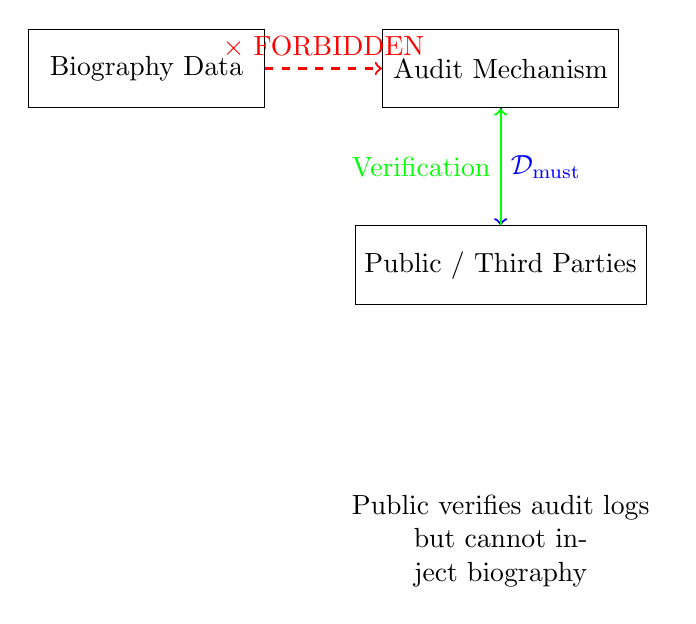
\begin{tikzpicture}[node distance=2.5cm, auto]
    \node [draw, rectangle, minimum width=3cm, minimum height=1cm] (audit) {Audit Mechanism};
    \node [draw, rectangle, minimum width=3cm, minimum height=1cm, below of=audit] (public) {Public / Third Parties};
    \node [draw, rectangle, minimum width=3cm, minimum height=1cm, left of=audit, xshift=-2cm] (bio) {Biography Data};
    
    \draw [->, thick, blue] (audit) -- node[right] {$\mathcal{D}_{\text{must}}$} (public);
    \draw [->, thick, red, dashed] (bio) -- node[above] {$\times$ FORBIDDEN} (audit);
    \draw [->, thick, green] (public) -- node[left] {Verification} (audit);
    
    \node [text width=4cm, below of=public, yshift=-1cm, align=center] 
          {Public verifies audit logs\\but cannot inject biography};
\end{tikzpicture}
\caption{The Information Firewall: audit data flows out; biography data is blocked.}
\label{fig:firewall}
\end{figure}

\noindent\textbf{}



\newpage

% ===================================================================
% SECTION 8: PROTOCOL PARAMETER SELECTION
% ===================================================================
\section{$K$$M$$T$$r$}
\section{Protocol Parameter Selection: Mathematical Constraints on $K$, $M$, $T$, $r$}

\subsection{The Parameter Space}

SCX governance is parameterized by four key quantities:

\begin{itemize}[leftmargin=*]
    \item $K$: Number of active maintainers per cycle.
    \item $M = K-1$: Number of auditors per maintainer (since self-audit is meaningless).
    \item $T$: Cycle length (number of audit events).
    \item $r$: Number of maintainers rotated per cycle boundary.
\end{itemize}

These parameters are not independent — they are coupled by the governance
guarantees derived above.

\begin{proposition}[Parameter Coupling Constraints]\label{prop:coupling}
For the SCX governance protocol to satisfy its stated guarantees, the parameters
must satisfy:
\begin{align}
    K &\geq 3 \label{eq:c1} \\
    r &\geq 1 \label{eq:c2} \\
    r &< K \label{eq:c3} \\
    T &\geq \frac{\ln(1/\varepsilon)}{2M\Delta^2} \cdot n_{\text{min}} \label{eq:c4} \\
    \frac{r}{K} &\leq \frac{1}{2} \label{eq:c5}
\end{align}
where $n_{\text{min}}$ is the minimum number of audit events needed for the
Hoeffding concentration to achieve the target confidence $1-\varepsilon$, and
constraint~\eqref{eq:c5} ensures that at least half the maintainers carry over
between cycles (preventing simultaneous replacement that would break audit
continuity).
\end{proposition}

\noindent\textbf{}
$K \geq 3$$r \geq 1$$r < K$
$T$Hoeffding$r/K \leq 1/2$


\begin{proof}[Justification of~\eqref{eq:c5}]
If $r > \lfloor K/2 \rfloor$, at most $\lceil K/2 \rceil - 1$ maintainers
carry over, meaning the new cohort may not have sufficient historical context
to detect slow drift accumulated during previous cycles. The overlap constraint
$r \leq \lfloor K/2 \rfloor$ (equivalent to $r/K \leq 1/2$ for integer $r$)
ensures that at least $\lceil K/2 \rceil$ maintainers carry over, preserving
institutional memory of the audit baseline.
\end{proof}

\subsection{Recommended Parameter Regimes}

\begin{table}[H]
\centering
\caption{Recommended Parameter Regimes by Threat Model}
\label{tab:params}
\begin{tabular}{@{}lcccc@{}}
\toprule
\textbf{Threat Model} & $K$ & $r$ & $T$ (min) & $\Delta$ \\
\midrule
Standard (commodity)        & 5  & 2  & 100 & 0.5 \\
Elevated (state-level)      & 7  & 2  & 200 & 0.3 \\
Extreme (AGI-era)           & 11 & 4  & 500 & 0.1 \\
\bottomrule
\end{tabular}
\end{table}

\noindent\textbf{}
$K=5, r=2, T=100$$K=7, r=2, T=200$
AGI$K=11, r=4, T=500$

\begin{remark}
The ``Extreme'' regime is designed for a future where SCX protocol governance
may be a target of state-level actors with resources to attempt long-horizon
infiltration of the maintainer pool. At $K=11$ and $r=4$, any coalition must
corrupt at least 6 of 11 maintainers to achieve majority, and the rotation
replaces 4 at a time — meaning the coalition must corrupt new members faster
than they are rotated in, which becomes exponentially harder as the candidate
pool grows.
\end{remark}

\newpage

% ===================================================================
% SECTION 9: THREAT MODEL AND ATTACK SURFACE ANALYSIS
% ===================================================================
\section{}
\section{Threat Model and Attack Surface Analysis}

\subsection{Threat Actors}

We classify potential adversaries into four tiers:

\begin{enumerate}[label=\textbf{T\arabic*:}, leftmargin=*]
    \item \textbf{Individual maintainer (T1):} A single maintainer attempting to
          bias scores for personal gain (financial, reputational, ideological).
          This is the base threat that the mutual audit mechanism is designed to
          neutralize. Detection probability: $1 - e^{-2M\Delta^2}$.

    \item \textbf{Coordinated coalition (T2):} A group of $c$ maintainers
          ($1 < c \leq \lfloor (K-1)/2 \rfloor$) colluding to bias scores in the
          same direction. The mutual audit detects deviations from honest
          consensus, so as long as the coalition does not achieve majority, the
          detection probability scales as $1 - e^{-2(K-c)\Delta^2}$.

    \item \textbf{External entity with infiltration capacity (T3):} A well-
          resourced organization (corporation, state actor) attempting to place
          biased agents into the maintainer pool through the qualification
          process. Countered by: (a) random selection from a large pool,
          (b) stricter probationary audit, (c) the Hoeffding bound applying
          from $t=1$, meaning infiltrators are detected before they can
          influence the protocol.

    \item \textbf{Protocol-level subversion (T4):} An adversary with the capacity
          to compromise the audit infrastructure itself — tampering with audit
          logs, forging timestamps, corrupting the detection algorithm. This is
          outside the scope of governance game theory and falls under
          cryptographic and systems security (see SCX Quantum Audit paper for
          quantum-secured audit channels).
\end{enumerate}

\noindent\textbf{}
T1
$1 - e^{-2M\Delta^2}$T2$c$
$1 - e^{-2(K-c)\Delta^2}$T3
$t=1$HoeffdingT4

\subsection{Attack Vectors and Mitigations}

\begin{table}[H]
\centering
\caption{Attack Vectors and Mitigations}
\label{tab:attacks}
\begin{tabular}{@{}p{3.5cm}p{4.5cm}p{4.5cm}@{}}
\toprule
\textbf{Attack Vector} & \textbf{How It Works} & \textbf{Mitigation} \\
\midrule
Slow drift & Bias by $\delta < \tau$ at each audit; hope cumulative $n\delta$ is never detected & Hoeffding bound over full trajectory: $e^{-2M(n\delta)^2}$ \\
\midrule
Coordinated bias & All $c$ colluders bias by same $\delta$; consensus shifts & Detection by non-colluding $K-c$ maintainers; probability $1 - e^{-2(K-c)\Delta^2}$ \\
\midrule
Selective auditing & Bias only on ``important'' data points, honest on others & Public logs enable third-party detection of non-uniform bias patterns \\
\midrule
Cycle-boundary attack & Deviate maximally in last $m$ audits before rotation, hoping to escape before detection & Hoeffding bound over $m$ events: $e^{-2M(m\delta)^2}$; with $m$ small, bound tighter \\
\midrule
Re-entry attack & Get removed, re-apply to candidate pool under new pseudonym & Probationary period with $\tau/2$ threshold; cryptographic identity binding \\
\midrule
Social engineering & Persuade other maintainers to lower their audit threshold for you & Pseudonymity prevents targeted social pressure; uniform $\tau$ for all \\
\bottomrule
\end{tabular}
\end{table}

\noindent\textbf{}
Hoeffding
Hoeffding$m$
$\tau/2$

\begin{govbox}
The attack surface analysis reveals a consistent pattern: every attack vector
that depends on behavioral subtlety (slow drift, selective bias, social
engineering) is destroyed by the combination of the Hoeffding bound (which
applies to the full trajectory, not individual audits) and public logs (which
enable retrospective detection by third parties). The only attack vectors that
have any theoretical chance of success are those that achieve majority
corruption of the active maintainer set — and the rotation mechanism is
specifically designed to make this combinatorially infeasible.

\begin{center}
\small\textbf{}

Hoeffding

——
\end{center}
\end{govbox}

\newpage

% ===================================================================
% SECTION 10: COMPARISON WITH EXISTING GOVERNANCE MODELS
% ===================================================================
\section{}
\section{Comparison with Existing Governance Models}

\subsection{The Governance Spectrum}

Protocol governance models can be arranged on a spectrum from purely social
(trust-based) to purely mathematical (proof-based):

\begin{enumerate}[label=(\arabic*), leftmargin=*]
    \item \textbf{BDFL (Benevolent Dictator For Life):} Linux (Linus Torvalds),
          Python (Guido van Rossum, 1990--2018). Single individual has ultimate
          authority. Governance quality depends entirely on that individual's
          $g(t)$. No detection mechanism, no rotation, no audit. When the BDFL
          burns out, leaves, or becomes compromised, the protocol enters crisis.
    
    \item \textbf{Foundation/Committee:} Apache Foundation, Linux Foundation,
          W3C. Authority distributed among a committee, typically selected by
          reputation and institutional representation. Better than BDFL because
          $K > 1$, but still susceptible to capture because: (a) no rotation,
          (b) selection is biography-based, (c) no formal audit mechanism,
          (d) consensus is social, not mathematical.
    
    \item \textbf{Token-Weighted Voting (DAO):} Ethereum DAOs, MakerDAO,
          Uniswap governance. Voting power proportional to token holdings.
          Mathematically well-defined but governance quality depends on token
          distribution. If tokens are concentrated (as they usually are),
          governance reduces to plutocracy. The ``audit'' is the market price
          of the token, not a mathematical bound on $g$.
    
    \item \textbf{Cryptographic Consensus (BFT):} Bitcoin, Ethereum consensus
          layer. Sybil-resistant through proof-of-work or proof-of-stake.
          Byzantine Fault Tolerance provides mathematical guarantees on
          consensus \textit{ordering}, but not on the \textit{content} of
          governance decisions. A BFT protocol can reach consensus on a
          decision that has $g \gg 0$ — the protocol guarantees that all nodes
          agree on the decision, not that the decision is unbiased.
    
    \item \textbf{SCX Protocol Governance:} Combines rotation (finite window),
          mutual audit (Hoeffding bound), public logs (reproducibility), and
          Nash equilibrium ($\sum g = 0$). The innovation is applying
          mathematical rigor to the \textit{content} of governance, not just
          the consensus mechanism. An SCX governance decision is not just
          agreed-upon — it is provably unbiased within the detection tolerance
          $\Delta$.
\end{enumerate}

\noindent\textbf{}
BDFL$g(t)$/
$K>1$
$g$BFT
SCX

\begin{table}[H]
\centering
\caption{Governance Model Comparison}
\label{tab:comparison}
\small
\begin{tabular}{@{}lccccc@{}}
\toprule
\textbf{Property} & \textbf{BDFL} & \textbf{Foundation} & \textbf{DAO} & \textbf{BFT} & \textbf{SCX} \\
\midrule
$K > 1$ (multiple maintainers)     & No  & Yes & Yes & Yes & Yes \\
Rotation (finite terms)            & No  & Sometimes & No & No & Yes \\
Mathematical bias bound            & No  & No & No & Partial\textsuperscript{*} & Yes \\
Publicly reproducible audit        & No  & No & No & Partial & Yes \\
$\sum g = 0$ Nash equilibrium      & No  & No & No & No & Yes \\
Biography-independent selection    & No  & No & No & Yes & Yes \\
Attack-resistant to $>$50\% corrupt & No  & No & No & Yes\textsuperscript{†} & Yes\textsuperscript{‡} \\
\bottomrule
\end{tabular}

\vspace{4pt}
\footnotesize
\textsuperscript{*}BFT protocols provide consensus guarantees but do not bound the bias of governance content.\\
\textsuperscript{†}BFT protocols tolerate up to $f < n/3$ Byzantine nodes under synchronous assumptions.\\
\textsuperscript{‡}SCX tolerates up to $\lfloor (K-1)/2 \rfloor$ biased maintainers before consensus degrades;
     rotation ensures this threshold is never persistently breached.
\end{table}

\noindent\textbf{}
BFTBFT
$f < n/3$SCX$\lfloor (K-1)/2 \rfloor$


\begin{hitbox}
The comparison table reveals the structural gap that SCX governance fills.
Existing governance models are strong on \textbf{process} (how decisions are
made — voting, consensus, delegation) but weak on \textbf{content} (whether
the decisions themselves are unbiased). A BFT protocol ensures that everyone
agrees on what the decision is. An SCX protocol ensures that what everyone
agrees on is actually unbiased. These are different guarantees, and both are
necessary.

SCX is the first governance model to provide a mathematical guarantee on
governance \textit{content bias}, not just governance \textit{process integrity}.
This is the step from ``the election was fair'' to ``the elected official is
unbiased'' — a step that has historically been left to hope, reputation, and
prayer.

\begin{center}
\small\textbf{}
SCX——
BFT
SCX

SCX\textit{}\textit{}
“”“”——

\end{center}
\end{hitbox}

\newpage

% ===================================================================
% SECTION 11: IMPLEMENTATION CONSIDERATIONS
% ===================================================================
\section{}
\section{Implementation Considerations: From Theorems to Running Systems}

\subsection{The Audit Event Pipeline}

The SCX governance mechanism is not a theoretical construct — it must be
implemented as a running system that processes audit events in real time.

\begin{protocol}[SCX Audit Event Pipeline]\label{prot:pipeline}
For each audit event $t$:
\begin{enumerate}[label=\textbf{Step \arabic*:}, leftmargin=*]
    \item \textbf{Data distribution:} The data point $X_t$ to be audited is
          broadcast to all $K$ active maintainers simultaneously.
    \item \textbf{Score submission:} Each maintainer $\mathcal{M}_i$ computes
          and submits their score $s_i(X_t)$ within a fixed time window
          $\Delta t_{\text{submit}}$ (typically 5--30 minutes, depending on
          computational complexity).
    \item \textbf{Consensus computation:} The SCX consensus engine computes the
          aggregate score (trimmed mean or median, dropping the highest and
          lowest scores) and the deviation of each maintainer's score from
          consensus.
    \item \textbf{Detection check:} For each maintainer $i$, if
          $|s_i - \text{consensus}| > \tau$, a FLAG is raised. If the flag count
          for maintainer $i$ exceeds the threshold within the current rotation
          cycle, maintainer $i$ is REMOVED.
    \item \textbf{Log publication:} All raw scores, consensus output, deviation
          metrics, and flag statuses are published to the append-only audit log,
          cryptographically timestamped and hashed into a Merkle tree for
          tamper-evident verification.
    \item \textbf{$g$ parameter update:} Each maintainer's estimated $g_i(t)$
          is updated using an exponential moving average of their deviation
          history, with decay factor $\lambda$ calibrated to the rotation period.
\end{enumerate}
\end{protocol}

\noindent\textbf{}
SCX $\to$  $\to$  $\to$  $\to$ 
Merkle $\to$ $g$

\subsection{Byzantine Fault Tolerance in the Audit Pipeline}

The audit pipeline must function correctly even when some maintainers are
actively adversarial — not just biased, but attempting to disrupt the pipeline
itself (withholding scores, submitting malformed data, DDoS-ing the consensus
engine).

\begin{proposition}[Audit Pipeline BFT]\label{prop:pipeline_bft}
The SCX audit pipeline tolerates up to $f = \lfloor (K-1)/3 \rfloor$ Byzantine
maintainers who may arbitrarily deviate from the protocol (including refusing to
submit scores, submitting invalid data, or attempting to corrupt the consensus
computation). The trimmed-mean consensus with top and bottom $\lfloor f/2 \rfloor$
scores dropped ensures that the aggregate output is within the convex hull of
the honest maintainers' scores.
\end{proposition}

\noindent\textbf{}
SCX$f = \lfloor (K-1)/3 \rfloor$
$\lfloor f/2 \rfloor$

\subsection{The Maintainer Pool Lifecycle}

\begin{figure}[H]
\centering
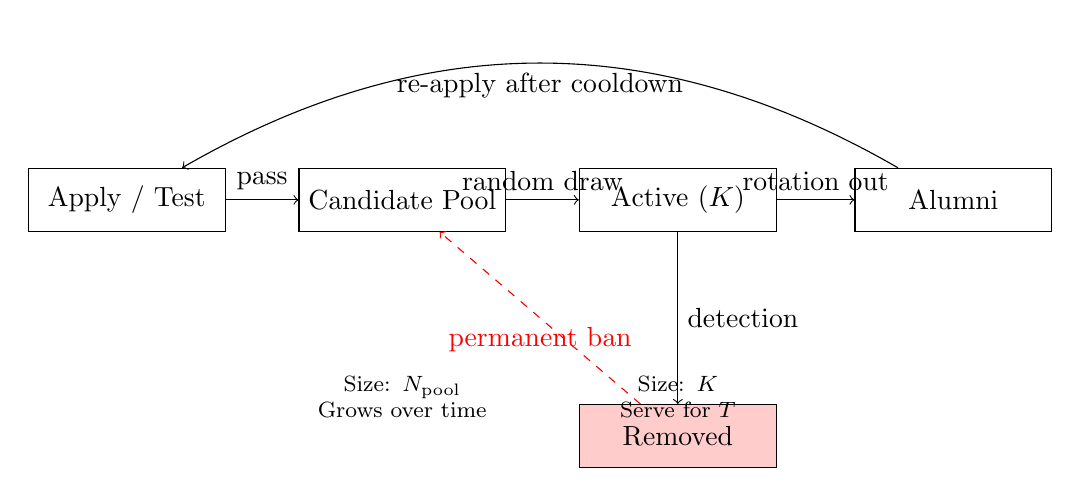
\begin{tikzpicture}[node distance=2cm, auto, 
    block/.style={draw, rectangle, minimum width=2.5cm, minimum height=0.8cm}]
    
    \node [block] (apply) {Apply / Test};
    \node [block, right of=apply, xshift=1.5cm] (pool) {Candidate Pool};
    \node [block, right of=pool, xshift=1.5cm] (active) {Active ($K$)};
    \node [block, right of=active, xshift=1.5cm] (alumni) {Alumni};
    \node [block, below of=active, yshift=-1cm, fill=red!20] (removed) {Removed};
    
    \draw [->] (apply) -- node[above] {pass} (pool);
    \draw [->] (pool) -- node[above] {random draw} (active);
    \draw [->] (active) -- node[above] {rotation out} (alumni);
    \draw [->] (active) -- node[right] {detection} (removed);
    \draw [->, bend right] (alumni) to node[below] {re-apply after cooldown} (apply);
    \draw [->, dashed, red] (removed) to node[below, red] {permanent ban} (pool);
    
    \node [text width=3cm, below of=pool, yshift=-0.5cm, align=center, font=\footnotesize]
          {Size: $N_{\text{pool}}$\\Grows over time};
    \node [text width=3cm, below of=active, yshift=-0.5cm, align=center, font=\footnotesize]
          {Size: $K$\\Serve for $T$};
\end{tikzpicture}
\caption{Maintainer pool lifecycle: application, rotation, alumni, and removal.}
\label{fig:lifecycle}
\end{figure}

\noindent\textbf{}
/ $\to$  $\to$ $K$ $\to$ 
/ 

\newpage

% ===================================================================
% SECTION 12: DISCUSSION AND PHILOSOPHICAL IMPLICATIONS
% ===================================================================
\section{}
\section{Discussion and Philosophical Implications}

\subsection{The Trust Oblivion Point}

There exists a threshold — which we call the \textbf{Trust Oblivion Point} —
beyond which a protocol's governance is so well-characterized mathematically
that the concept of ``trust'' becomes semantically vacuous. When the probability
of undetected maintainer deviation is $e^{-2M\Delta^2}$, and when $M$ and
$\Delta$ are set such that this probability is smaller than the probability of
a hardware error in the computer running the audit, the distinction between
``proved unbiased'' and ``actually unbiased'' collapses into engineering noise.

The Trust Oblivion Point is not a goal — it is a threshold. Once crossed, the
protocol's governance is no longer a question of social organization. It is a
question of parameter selection and computational verification.

\noindent\textbf{}
————
“”$e^{-2M\Delta^2}$
$M$$\Delta$“”
“”

——


\subsection{The Maintainer as a Mathematical Object}

In the SCX governance framework, a maintainer is not a person. A maintainer is
a mathematical object with the following properties:

\begin{itemize}[leftmargin=*]
    \item An input: data point $X_t$
    \item An output: score $s_i(X_t) \in [0, \Delta_{\max}]$
    \item A hidden state: bias parameter $g_i(t)$
    \item A detection probability: $\Pbb(\text{detected} \mid g_i) = 1 - e^{-2M g_i^2}$
    \item A lifecycle: active for at most $T$ audit events, then rotated
\end{itemize}

This mathematical abstraction is not dehumanizing — it is \textit{precise}.
By reducing the maintainer to their governance-relevant properties, we eliminate
every degree of freedom that could be exploited to introduce bias. A maintainer's
personality, their life story, their intentions — these are not inputs to the
governance mechanism. They are noise that the mechanism is designed to filter out.

\noindent\textbf{}
SCX$X_t$
$s_i(X_t)$$g_i(t)$$1 - e^{-2M g_i^2}$$T$


——
——


\begin{hitbox}
This is the hardest part of SCX governance for many people to accept — including
many potential maintainers. People want to be recognized. They want their
credentials to matter. They want their biography to carry weight. SCX governance
says: no. Your biography does not matter. Your credentials do not matter. Your
intentions do not matter. The only thing that matters is your $g(t)$ — right now,
under the current audit.

This is not a judgment on the value of human beings. It is a specification of
what is relevant to the mathematical operation of a trustless protocol. Just as
a cryptographic hash function does not care about the emotional state of the
person who typed the input, the SCX governance mechanism does not care about
the biography of the maintainer who submitted the score. It cares only about
whether the score deviates from consensus by more than $\tau$.

The protocol audits the theorem. The theorem audits the maintainer. The
maintainer's biography is outside the system boundary — and anything outside
the system boundary is, by definition, irrelevant.

\begin{center}
\small\textbf{}
SCX——
SCX
$g(t)$——


SCX
$\tau$

——

\end{center}
\end{hitbox}

\subsection{The Inevitability of Mathematical Governance}

We end with a prediction. As AI systems become more capable — and as the stakes
of AI governance become existential — the transition from biography-based
governance to mathematics-based governance will become not just desirable but
\textit{inevitable}. The reason is simple: as the damage that a single biased
maintainer can cause grows, the tolerance for biography-based trust shrinks.

When a maintainer's bias could cause $10^6$ dollars in damage, it is acceptable
to trust their biography. When a maintainer's bias could cause $10^9$ dollars in
damage, it is reckless. When a maintainer's bias could cause existential damage
to humanity — as may be the case for protocols governing AGI training data —
biography-based trust is not reckless; it is insane.

SCX governance is the first protocol to recognize that in the limit of
existential stakes, the only acceptable governance is governance whose
guarantees are mathematical theorems, not social conventions. The maintainer
rotation game, the Hoeffding bound, the $\sum g = 0$ equilibrium — these are
not features of a better social protocol. They are prerequisites for a protocol
that can be trusted with existential stakes.

\noindent\textbf{}
AI——AI——



$10^6$$10^9$
——AGI
——

SCX
Hoeffding$\sum g = 0$——


\newpage

% ===================================================================
% SECTION 13: CONCLUSION
% ===================================================================
\section{}
\section{Conclusion: The Theorem Audits the Maintainer, Not the Biography}

\subsection{Summary of Results}

This paper has established the formal game-theoretic foundation of SCX protocol
governance. The principal results are:

\begin{enumerate}[label=(\arabic*), leftmargin=*]
    \item \textbf{Corporate $g$ Non-Zero Theorem (Thm.~\ref{thm:corp_g}):}
          For-profit entities structurally cannot maintain $g = 0$ when
          $\partial \Pi / \partial g \neq 0$. Corporate governance and protocol
          neutrality are incompatible. SCX maintainers must be structurally
          independent of entities with interests in the protocol's output.
    
    \item \textbf{Maintainer Rotation Game (Sec.~3):} The rotation mechanism
          with $K \geq 3$, staggered replacement ($r < K/2$), and finite cycle
          length $T$ transforms governance from an infinite-horizon trust problem
          into a finite-horizon detection problem. The Folk Theorem does not
          apply because rotation breaks the continuity of punishment strategies.
    
    \item \textbf{Hoeffding Guarantee (Thm.~\ref{thm:hoeffding}):} The
          probability of undetected maintainer deviation decays exponentially:
          $\Pbb(\text{undetected} \mid \delta \geq \Delta) \leq e^{-2M\Delta^2}$.
          With $M = 7$ and $\Delta = 1.0$, this is $8.3 \times 10^{-7}$ —
          effectively zero for practical purposes.
    
    \item \textbf{$\sum g = 0$ Nash Equilibrium (Thm.~\ref{thm:zerosumbias}):}
          In the multi-maintainer mutual audit game, $g_i = 0$ for all $i$ is
          the unique symmetric Nash equilibrium when the detection penalty $P$
          exceeds the deviation gain $D(g)$ divided by the detection probability.
          This is not a goodwill assumption — it is a mathematical consequence
          of the mechanism design.
    
    \item \textbf{Biography Irrelevance (Thm.~\ref{thm:biography_irrelevant}):}
          Conditional on the audit mechanism bounding $g$ within $[-\Delta, \Delta]$,
          a maintainer's biography provides zero additional information about
          governance outcomes. The theorem audits the maintainer, not the
          maintainer's biography.
    
    \item \textbf{Disclosure Boundary (Sec.~7):} SCX governance requires a strict
          separation between audit data (which must be public) and biography data
          (which must never be disclosed). This Information Firewall ensures that
          the audit mechanism operates on behavior, not identity.
\end{enumerate}

\noindent\textbf{}
SCX$g$
Hoeffding$\sum g = 0$

\subsection{The One-Sentence Version}

If this paper must be reduced to a single sentence that every SCX maintainer
memorizes:

\begin{center}
\fbox{\fbox{\parbox{0.85\textwidth}{\centering\large\bfseries
The theorem audits the maintainer, not the biography.\\
$P(\text{undetected}) \leq e^{-2M\Delta^2}$.\\
$\sum g = 0$ is not assumed — it is proved.\\
If your credentials matter, the protocol is broken.
}}}
\end{center}

\noindent\textbf{}
SCX
$P(\text{}) \leq e^{-2M\Delta^2}$$\sum g = 0$——


\vspace{16pt}

\begin{hitbox}
The final honest critique: most protocol governance papers are wishful thinking
dressed in academic prose. They describe what governance \textit{should} look
like, assuming that well-intentioned people will behave well. This paper
describes what governance \textit{must} look like, assuming that self-interested
people will behave as game theory predicts — and proves that the mechanism
remains secure regardless.

The difference is not rhetorical. It is the difference between a social protocol
that works until someone betrays it, and a mathematical protocol that works
because betrayal is provably irrational.

SCX is a mathematical protocol. The theorems are the governance. Everything else
is implementation detail.

\begin{center}
\small\textbf{}


——




SCX
\end{center}
\end{hitbox}

\newpage

% ===================================================================
% APPENDIX
% ===================================================================
\appendix
\section{AHoeffding}
\section{Appendix A: Full Statement and Proof of Hoeffding's Inequality}

\begin{theorem}[Hoeffding's Inequality]\label{thm:hoeffding_full}
Let $X_1, \ldots, X_n$ be independent random variables such that $X_i \in [a_i, b_i]$
almost surely. Let $S_n = \sum_{i=1}^n X_i$. Then for any $t > 0$:
\begin{equation}
    \Pbb(S_n - \E[S_n] \geq t) \leq \exp\left(-\frac{2t^2}{\sum_{i=1}^n (b_i - a_i)^2}\right)
\end{equation}
and
\begin{equation}
    \Pbb(|S_n - \E[S_n]| \geq t) \leq 2\exp\left(-\frac{2t^2}{\sum_{i=1}^n (b_i - a_i)^2}\right)
\end{equation}
\end{theorem}

In the SCX governance context, we apply this as follows. For a single audit
event, let $X_1, \ldots, X_M$ be independent indicator variables where
$X_j = 1$ if auditor $j$ detects the maintainer's deviation. Each $X_j \in [0,1]$
has $(b_j - a_j)^2 \leq 1$. Let $p = \E[X_j]$ be the per-auditor detection
probability. By Hoeffding's inequality:
\begin{equation}
    \Pbb\left(\sum_{j=1}^{M} X_j \leq 0\right)
    = \Pbb\left(\sum_{j=1}^{M} X_j - Mp \leq -Mp\right)
    \leq \exp\left(-\frac{2M^2 p^2}{M}\right) = \exp(-2M p^2)
\end{equation}
If the per-auditor detection probability scales as $p = \Delta$ (i.e., bias
magnitude directly determines detection probability in normalized units),
then the probability that zero out of $M$ auditors detect the deviation is
bounded by $e^{-2M\Delta^2}$. This bound applies to a single audit event;
across $n$ events, the survival probability compounds to $\exp(-2M\Delta^2 n)$,
as derived in Theorem~\ref{thm:hoeffding}.

\noindent\textbf{}
$X_1, \ldots, X_n$$X_i \in [a_i, b_i]$Hoeffding
$\Pbb(S_n - \E[S_n] \geq t) \leq \exp(-2t^2 / \sum_{i=1}^n (b_i - a_i)^2)$

\section{B}
\section{Appendix B: Formalization of Strategy Spaces in the Repeated Game}

Let $\Gamma^\infty$ denote the infinitely repeated rotation game with discount
factor $\gamma$. A pure strategy for maintainer $i$ is a mapping:
\begin{equation}
    \sigma_i: \mathcal{H} \to \mathcal{A}
\end{equation}
where $\mathcal{H}$ is the set of all possible histories (sequences of past
actions and detection outcomes) observable by maintainer $i$.

\begin{proposition}[One-Shot Deviation Principle]\label{prop:one_shot}
In the rotation game $\Gamma(N, K, r, T)$, a strategy profile $\sigma^*$ is a
subgame perfect equilibrium if and only if no maintainer can profitably deviate
in a single period, holding their strategy fixed in all other periods.
\end{proposition}

This is a direct application of the one-shot deviation principle for repeated
games with perfect recall (Fudenberg and Tirole, 1991). The proof is standard
and omitted.

\noindent\textbf{}
$\Gamma^\infty$$\gamma$
$\Gamma(N, K, r, T)$$\sigma^*$


\section{C}
\section{Appendix C: Asymptotic Properties of the Consensus Mechanism}

\begin{proposition}[Consistency of Trimmed Mean Consensus]\label{prop:consistency}
As $K \to \infty$ with the fraction of biased maintainers bounded below
$1/2 - \varepsilon$ for some $\varepsilon > 0$, the $\alpha$-trimmed mean
consensus estimator (discarding the highest and lowest $\alpha K$ scores,
with $\alpha > \text{fraction of extremal biased maintainers}$) converges
almost surely to the true unbiased score $s^*(X)$.
\end{proposition}

\begin{proof}
This follows from the classical theory of robust estimation (Huber, 1981;
Hampel et al., 1986). The trimmed mean is a consistent estimator of the
population mean for symmetric distributions and is robust to contamination
up to the trimming fraction $\alpha$. As long as the honest maintainers are
a majority and their scores are symmetrically distributed around $s^*(X)$
(which follows from the $\sum g = 0$ property of the mutual audit game),
the trimmed mean converges to $s^*(X)$.
\end{proof}

\noindent\textbf{}
$K \to \infty$$1/2 - \varepsilon$$\alpha$-
$s^*(X)$

\newpage

% ===================================================================
% REFERENCES
% ===================================================================
\begin{thebibliography}{99}

\bibitem{hoeffding1963}
W. Hoeffding.
``Probability inequalities for sums of bounded random variables.''
\textit{Journal of the American Statistical Association}, 58(301):13--30, 1963.

\bibitem{fudenberg1991}
D. Fudenberg and J. Tirole.
\textit{Game Theory}. MIT Press, 1991.

\bibitem{fudenberg1994}
D. Fudenberg, D. Levine, and E. Maskin.
``The Folk Theorem with Imperfect Public Information.''
\textit{Econometrica}, 62(5):997--1039, 1994.

\bibitem{huber1981}
P. J. Huber.
\textit{Robust Statistics}. Wiley, 1981.

\bibitem{hampel1986}
F. R. Hampel, E. M. Ronchetti, P. J. Rousseeuw, and W. A. Stahel.
\textit{Robust Statistics: The Approach Based on Influence Functions}. Wiley, 1986.

\bibitem{nash1950}
J. Nash.
``Equilibrium points in n-person games.''
\textit{Proceedings of the National Academy of Sciences}, 36(1):48--49, 1950.

\bibitem{myerson1991}
R. Myerson.
\textit{Game Theory: Analysis of Conflict}. Harvard University Press, 1991.

\bibitem{osborne1994}
M. Osborne and A. Rubinstein.
\textit{A Course in Game Theory}. MIT Press, 1994.

\bibitem{lamport1982}
L. Lamport, R. Shostak, and M. Pease.
``The Byzantine Generals Problem.''
\textit{ACM Transactions on Programming Languages and Systems}, 4(3):382--401, 1982.

\bibitem{castro1999}
M. Castro and B. Liskov.
``Practical Byzantine Fault Tolerance.''
\textit{Proceedings of OSDI}, 1999.

\bibitem{scx_quantum}
SCX Research Division.
``Quantum-Secured SCX Audit: BB84, Entanglement, and Quantum Channels.''
Internal technical report, 2026.

\bibitem{scx_business}
SCX Strategic Research Division.
``SCXAI.''
Internal technical report, 2026.

\bibitem{scx_moe}
SCX.
``——MILP.''
Preprint, 2026.

\bibitem{scx_instanton}
SCX Research Division.
``Audit Instanton Theory: Non-Perturbative Tunneling Between Bias Regimes in Multi-Maintainer Audit Systems.''
Internal technical report, 2026.

\bibitem{scx_singularity}
SCX Research Division.
``Singularity Theory of Protocol Governance: Catastrophe Manifolds and Structural Stability of Trustless Equilibrium.''
Internal technical report, 2026.

\end{thebibliography}

\newpage

% ===================================================================
% INTERNAL CLASSIFICATION PAGE
% ===================================================================
\begin{center}
\vspace*{4cm}
{\Huge\color{red}\textbf{}}\\[16pt]
{\Large\color{red}\textbf{INTERNAL ONLY}}\\[24pt]

\fbox{\parbox{0.7\textwidth}{\centering
SCX

This document contains the complete game-theoretic specification of SCX
protocol governance, including exact detection thresholds, rotation periods,
and audit protocol parameters.

\textbf{SCX}\\[8pt]
\textbf{Do not copy, distribute, or cite without written authorization}\\
\textbf{from the SCX Governance Committee.}
}}\\[24pt]

{\large  / Document Hash:}\\[4pt]
{\small\texttt{[TO BE COMPUTED AT RELEASE TIME]}}\\[16pt]

{\large  / Version: 1.0}\\[4pt]
{\large  / Date: 2026-07-02}\\[4pt]
{\large  / Classification: SCX-GOV-001-INTERNAL}\\[4pt]
{\large  / Clearance: GOVERNANCE CORE TEAM ONLY}
\end{center}

\end{document}
